\documentclass[12pt, a4paper]{report}
\special{papersize=210mm, 297mm}
\usepackage[romanian]{babel}
\usepackage[utf8x]{inputenc}
\usepackage[left=2.5cm, right=2.5cm, top=2.5cm]{geometry}
\renewcommand{\baselinestretch}{1.4}
\usepackage[toc,page]{appendix}

\usepackage{amsmath}
\usepackage{graphicx}
\usepackage{float}
\graphicspath{{images/} {diagrams/}}

\usepackage{fullpage}
\usepackage{hyperref}
\usepackage{url}
\usepackage{listings}
\usepackage{verbatim}
\usepackage{color}
\usepackage{listings}
\usepackage{xcolor}

\definecolor{codegreen}{rgb}{0,0.6,0}

\lstset{frame=tb,
	 language=java,
	showstringspaces=false,
	columns=flexible, basicstyle={\small\ttfamily},
	numbers=none, numberstyle=\tiny\color{gray},
	keywordstyle=\color{blue},
	commentstyle=\color{dkgreen},
	stringstyle=\color{codegreen},
	morecomment=[f][\color{green}][0]{/},
	breakatwhitespace=true,
	tabsize=3
}

\usepackage{multirow}
\usepackage{array}
\newcolumntype{L}[1]{> {\raggedright\let\newline\\\arraybackslash\hspace{0pt}}m{#1}}
\newcolumntype{C}[1]{>{\centering\let\newline\\\arraybackslash\hspace{0pt}}m{#1}}
\newcolumntype{R}[1]{>{\raggedleft\let\newline\\\arraybackslash\hspace{0pt}}m{#1}}

\pagenumbering{roman}

\begin{document}

%======================================================================

\begin{titlepage}

	\newcommand{\HRule}{\rule{\linewidth}{0.5mm}} % Defines a new command for the horizontal lines, change thickness here

	\center % Center everything on the page

	%----------------------------------------------------------------------------------------
	%	LOGO SECTION
	%----------------------------------------------------------------------------------------

	\vspace{-20pt}
	
\includegraphics[width=100pt]{FMI-03.png}\\[1.0cm] % Include a department/university logo - this will require the graphicx package

	\textsc{\LARGE Universitatea de Vest din Timi\c{s}oara}\\[0.5cm] % Name of your university/college
	\textsc{\Large Facultatea de Matematic\u{a} \c{s}i Informatic\u{a}}\\[0.5cm] % Major heading such as course name
	\textsc{\large Domeniul de Studii: \\Informatic\u{a} Aplicat\u{a}}\\[3cm] % Minor heading such as course title

	%----------------------------------------------------------------------------------------
	%	TITLE SECTION
	%----------------------------------------------------------------------------------------

	\textsc{\Huge Lucrare de Diserta\c tie}\\[5cm]

	%\HRule \\[0.5cm]
	%{\huge \bfseries Simplified Transport Layer Security}
	%\\[0.4cm]
	%{\huge \bf implementation}\\[3cm] % Title of your document
	%\HRule \\[1.5cm]

	%----------------------------------------------------------------------------------------
	%	AUTHOR SECTION
	%----------------------------------------------------------------------------------------

	\begin{minipage}{0.4\textwidth}
		\begin{flushleft} \large
			\textbf{COORDONATOR:}\\
			Conf. Dr. Cristina \textsc{M\^ indru\c t\u a } % Coordinator
		\end{flushleft}
	\end{minipage}
	~
	\begin{minipage}{0.4\textwidth}
		\begin{flushright} \large
			\textbf{ABSOLVENT:} \\
			Nicolae \textsc{Savilencu} % Student's Name
		\end{flushright}
	\end{minipage}\\[1cm]


	%----------------------------------------------------------------------------------------
	%	DATE SECTION
	%----------------------------------------------------------------------------------------
	\vfill
	{\large Timi\c{s}oara \\2023}\\ % Date, change the \today to a set date if you want to be precise


	%----------------------------------------------------------------------------------------

	%\vfill % Fill the rest of the page with whitespace

\end{titlepage}

% =====================================================================

% second title page. as requested by UVT

\begin{titlepage}

	\newcommand{\HRule}{\rule{\linewidth}{0.5mm}} % Defines a new command for the horizontal lines, change thickness here

	\center % Center everything on the page

	%----------------------------------------------------------------------------------------
	%	LOGO SECTION
	%----------------------------------------------------------------------------------------

	%\vspace{-20pt}
	%
\includegraphics[width=100pt]{FMI-03.png}\\[1.0cm] % Include a department/university logo - this will require the graphicx package

	\textsc{\LARGE Universitatea de Vest din Timișoara}\\[0.5cm] % Name of your university/college
	\textsc{\Large Facultatea de Matematică și Informatică}\\[0.5cm] % Major heading such as course name
	% \textsc{\large Domeniul de Studii: \\Informatică Aplicată}\\[6cm] % Minor heading such as course title

	%----------------------------------------------------------------------------------------
	%	TITLE SECTION
	%----------------------------------------------------------------------------------------

	%\textsc{\Huge Master Dissertation}\\[2cm]

	\HRule \\[0.5cm]
	{\Huge \bf Tehnologii de randare a informa\c tiilor \^ in aplica\c tiile web moderne}\\[6cm] % Title of your document
	%\HRule \\[1.5cm]

	%----------------------------------------------------------------------------------------
	%	AUTHOR SECTION
	%----------------------------------------------------------------------------------------

	%\textsc{\huge Intermediate Report}

	\begin{minipage}{0.4\textwidth}
		\begin{flushleft} \large
			\textbf{COORDONATOR:}\\
			Conf. Dr. Cristina \textsc{M\^ indru\c t\u a} % Coordinator
		\end{flushleft}
	\end{minipage}
	~
	\begin{minipage}{0.4\textwidth}
		\begin{flushright} \large
			\textbf{ABSOLVENT:} \\
			Nicolae \textsc{Savilencu} % Student's Name
		\end{flushright}
	\end{minipage}\\[1cm]

	%----------------------------------------------------------------------------------------
	%	DATE SECTION
	%----------------------------------------------------------------------------------------
	\vfill
	{\large Timișoara\\ 2023}\\ % Date, change the \today to a set date if you want to be precise


	%----------------------------------------------------------------------------------------

	%\vfill % Fill the rest of the page with whitespace

\end{titlepage}

\begin{abstract}
	%The abstract should have one page and should be a compact presentation of the dissertation.
	\vspace{1.0cm}
	\par

	The web is evolving with high pace, and with the emergence of new web technologies, the way web applications are build has changed significantly, compared to the structures used in the past. Rendering is a critical aspect of web development, and modern web applications require faster, more efficient rendering techniques to deliver a better user experience. This dissertation aims to explore the rendering technologies used in modern web applications in order to define an optimal, yet flexible solution for developing applications of different scales.

	The research begins by introducing the fundamental concepts of web rendering, including two of the most known approaches: server-side rendering and client-side rendering. It then examines the evolution of rendering technologies, from traditional rendering techniques with HTML, CSS, and JavaScript, to modern technologies like React, Gatsby, Next. The dissertation compares and contrasts these technologies and analyzes their performance and usability by some predefined metrics: LCP (\emph{Largest Contentful Paint}), FID (\emph{First Input Delay}), CLS (\emph{Cumulative Layout Shift}), and other important factors such as development time and scalling ability.

	Dissertation explores the impact of rendering technologies on development workflows, examines the challenges associated with adopting new technologies, such as learning curve, compatibility issues, performance bottlenecks, and SEO optimization.

	Finally, the dissertation provides a case study of a web application build using multimple technologies, and comparing the performance metrics, individual technologies advantages and disadvantages.

	Overall, the dissertation provides a comprehensive analysis of rendering technologies in modern web applications and their impact on web development, to indentify most optimal methods of creating performant, scallable, and user friendly applications.


\end{abstract}

\tableofcontents{}
\addcontentsline{toc}{chapter}{Listă de figuri}
\listoffigures{}

\newpage{}

\chapter{Introducere}

\pagenumbering{arabic}
\setcounter{page}{1}


\section{Motivație și scop}

Obiectivul acestei lucrări este de a analiza tehnologiile de randare utilizate în aplicațiile web moderne, pentru a identifica metode de dezvoltare optime, din punct de vedere al performanței, experienței utilizatorului și SEO. Aceste rezultate vor fi obținute prin compararea mai multor framework-uri front-end după un anumit set de criterii, prestabilit. În urma comparării acestora, prin intermediu dezvoltării unei aplicații, se vor identifica cele mai eficiente șabloane de dezvoltare.

Motivația alegerii acestei teme de disertație derivă din mai mulți factori. În primul rând, progresul tehnologic rapid a dus la apariția mai multor paradigme de dezvoltare a aplicațiilor web, iar ținerea pasului cu acestea a devenit o provocare. În al doilea rând, odată cu crearea unor aplicații din ce în ce mai complexe, necesitatea de a cunoaște procesele interne precum tehnologiile și metodele de randare a devenit o componentă esențială a dezvoltării. Prin urmare, înțelegerea modului în care funcționează aceste tehnologii și a modului în care acestea pot fi optimizate poate ajuta la dezvoltarea unei aplicații care ar oferi o experiență de utilizare și o performanță sporită.

În cele din urmă, această lucrare de disertație își propune să ofere informații despe tehnologiile de randare utilizate în aplicațiile web moderne și despre impactul acestora asupra performanței, pentru a identifica cele mai eficiente framework-uri pentru a dezvolta o aplicație web ce poate fi scalată, bine optimizată și cu un user experience de nivel înalt.


\section{Contextul lucrării}


World Wide Web nu este un sinonim al internetului, dar este cea mai proeminentă parte a acestuia, care poate fi definită ca un sistem tehno-social cu care interacționează oamenii prin intermediul rețelelor tehnologice. Noțiunea de sistem tehno-social se referă la un sistem care îmbunătățește percepția umană, comunicarea și cooperarea. Percepția este condiția prealabilă necesară pentru a comunica și coopera. \cite{theoreticalfundationsoftheweb}

Pe 12 Martie 1989, Tim Berners-Lee, informatician de origine britanică și un fost angajat CERN au scris o propunere pentru ceea ce va deveni ulterior World Wide Web. Acea propunere avea drept scop crearea unui sistem de comunicații mai eficient în cadrul CERN, însă Berners-Lee a realizat în cele din urmă că conceptul ar putea fi implementat la scară globală. Împreună cu informaticianul belgian Robert Cailliau au propus în 1990 să folosesacă hypertext pentru a lega și accesa diverse tipuri de informații dintr-o rețea de noduri în care utilizatorul poate naviga către rezultatele dorite.

Prima versiune a web-ului global de la CERN a fost construit\u a pe primele versiuni ale HTTP (HyperText Transfer Protocol) \c si HTML (HyperText Markup Language). Aceste pagini web au fost servite de primul server web. Berners-Lee a scris, de asemenea, primul browser web pentru a accesa acest nou web creat. Web-ul global s-a schimbat drastic de la concep\c tia sa original\u a din 1989.

\subsection{Web 1.0}

A fost creat în 1989 și utilizat până în 2005. Potrivit lui Tim Berners-Lee Web 1.0 a fost \emph{read-only}, deoarece oferea foarte puțină interacțiune pentru utilizatori. Rolul web-ului a fost de natură pasaivă.

Web 1.0 a fost prima generație de World Wide Web și conținea doar pagini statice ce aveau doar un singur scop - de livrare a conținutului. Deoarece era monodirectional, \^ insemna c\u a organiza\c tiile \^ imp\u art\u a\c seau informa\c tii precum bro\c suri, cataloage \^ doar pentru citire. Aceste date erau prezentate pe pagini HTML statice care se modificau manual. Utilizatorii nu puteau contribui la paginile web existente. Tehnologiile Web 1.0 includ protocoale web de bază, HTML, HTTP și URI.

Browserele erau foarte rudimentare \c si site-urile web erau mici. De aceea era destul s\u a se creeze un fi\c sier HTML static care ar con\c tine toate datele necesare \c si designul, care nu ar fi fost niciodat\u a actualizate automat. A\c sa arat\u a un fi\c sier HTML:
\begin{lstlisting}
	!DOCTYPE html>
	<html>
		<head>
			<title>Page Title</title>
		</head>
		<body>
			<h1>Heading example</h1>
			<p>My first paragraph.</p>
		</body>
	</html>
\end{lstlisting}

Mai t\^ arziu, c\^ and browser-ele au dezvoltat capacit\u a\c ti vizuale, a aparut necesitatea de stilizare. Håkon W Lie a propus o prima versiune a CSS (Cascading Style Sheet), care este folosit \c si \^ in prezent. Un style sheet arat\u a astfel:
\begin{lstlisting}
	body {
		background-color: black;
	}

	p {
		font-size: 12px;
	}
\end{lstlisting}

\newpage
\textbf{Caracteristici:}
\begin{itemize}
	\item Conținut read-only
	\item Informațiile erau la dispoziția oricui și oricând
	\item Include pagini web statice și utilizează HTML
\end{itemize}


\textbf{Limitări:}
\begin{itemize}
	\item Paginile puteau fi înțelese doar de oameni și nu aveau conținut compatibil pentru motoare de căutare
	\item Utilizatorii erau responsabili pentru responsabili pentru actualizarea și gestionarea conținutului
	\item Incapabilitatea de a reprezenta informații dinamice
\end{itemize}

\subsection{Web 2.0}

A fost definit de Dale Dougherty în 2004. Tim O'Reilly a definit ulterior Web 2.0 astfel [66]:
"Web 2.0 este revolu\c tia afacerilor \^ in industria calculatorului, cauzat\u a de mutarea c\u atre internet ca platform\u a \c si \^ incercarea de a \^ in\c telege regulile pentru succes pe aceast\u a nou\u a platform\u a. Printre aceste reguli se num\u ar\u a urm\u atoarea: construirea de aplica\c tii care s\u a valorifice efectele de re\c tea pentru a deveni mai bune pe m\u asur\u a ce mai mul\c ti oameni le folosesc."

Web 2.0 facilitează proprietăți majore cum ar fi practicile participative, colaborative și distribuite, care permit desfășurarea activităților zilnice formale și în sfere formale pe web. Web 2.0 este web-as-a-platform. Utilizatorii au mai multe unelte pentru interacțiune, însă cu mai puțin control. Versiunea 2.0 implică și un design web flexibil, reutilizare creativă, actualizări și creare de conținut colaborativ, care este considerată una dintre cele mai remarcabile caracteristici ale web 2.0.

\^ Impreun\u a cu primele site-uri web dinamice a venit nevoia pentru primele tehnologii de programare pe partea de server. La \^ inceput, programarea pe partea de server se f\u acea direct \^ in serverul web. Mai t\^ arziu, standardul CGI (Common Gateway Interface) a fost dezvoltat, ceea ce a f\u acut posibil\u a interac\c tiunea serverului web cu orice proces local.
Mai t\^ arziu, limbi precum Perl, Java, PHP \c si ASP (\c si altele) au devenit populare pentru programare pe partea de server.

Site-urile web care devin mai bogate \^ in func\c tii au nevoie de mai mult\u a flexibilitate \c si de o utilizare mai bun\u a. Acesta este momentul \^ in care programarea client-side intr\u a \^ in joc. F\u ar\u a a fi nevoie de o \^ inc\u arcare complet\u a a paginii, con\c tinutul poate fi schimbat de c\u atre utilizatorii finali. Tehnologia cel mai utilizat\u a pentru acest scop este JavaScript.
C\^ and func\c tiile client-side au devenit \c si mai importante, au fost concepute framework-uri pentru renderizarea (\c si controlarea) paginilor client-side. Cele mai cunoscute framework-uri sunt: Ember, Angular \c si React.

\textbf{Caracteristici:}
\begin{itemize}
	\item Web-ul a devenit o platformă cu software peste nivelul unui singur dispozitiv
	\item Trecerea la internet-as-a-platform și încercarea de a înțelege regulile succesului în această nouă platformă
	\item Social Web este adesea folosit pentru a caracteriza site-urile care constau din comunități. Este bazat pe content management și identificarea unor noi metode de comunicare și interacționare dintre utilizatori. Aplicația web facilitează producerea colectivă de cunoștințe, rețele sociale și crește rata de schimb de informații dintre utilizatori
\end{itemize}


\textbf{Limitări:}
\begin{itemize}
	\item Ciclu constant de iterații a schimbarilor și actualizărilor serviciilor
	\item Probleme etice privind construirea și utilizarea web 2.0
	\item Interconectivitatea și schimbul de cunoștințe între platforme dincolo de granițele comunității sunt încă limitate
\end{itemize}

\subsection{Web 3.0}

Cunoscut și sub numele de web semantic sau Web decentralizat, este următoarea generație a World Wide Web, care își propune să ofere o experiență mai inteligentă, interconectată și decentralizată. Reprezintă o viziune pentru viitorul web în care datele, aplicațiile și serviciile sunt interconectate în mod fluid, permițând mașinilor și oamenilor să înțeleagă și să interacționeze mai eficient cu informațiile.

Ideea ce se află la bază este de a defini structurile de date și de a le lega pentru o automatizare, intregare și reutilizare mai eficientă în diverse aplicații. Web 3.0 este capabil să îmbunătățească gestionarea datelor, să susțină accesibilitatea internetului mobil, să stimuleze creativitatea și inovația, să încurajeze fenomenul de globalizare, să sporească experiența utilizatorilor și să ajute la organizarea colaborării în rețelele sociale.

În 3.0 conceptul de site web și pagină web dispare, datele nu sunt deținute, ci partajate, iar serviciile afișează diferite vederi, pe baza datelor. Aceste servicii pot fi aplicații și trebuie să se concentreze pe context și personalizare, ce vor fi atinse prin utilizarea căutarilor verticale. Web 3.0 facilitează dezvoltarea de aplicații care utilizează inteligența artificială, învățarea automată și procesarea limbajului natural. Aceste tehnologii permit analiza avansată a datelor, automatizarea și capacitatea de luare a deciziilor, rezultând în servicii mai inteligente și personalizate pentru utilizatori.

Urm\u atorul pas \^ in dezvoltarea web-ului este crearea aplica\c tiilor web autonome, care pot fi, de asemenea, utilizate f\u ar\u a conexiune la internet. Acestea sunt numite Aplica\c tii Web Progressive (PWA). Crearea acestor aplica\c tii nu este posibil\u a f\u ar\u a a avea control complet la nivelul clientului. Renderizarea pe partea de server nu este posibil\u a \c si se folosesc framework-uri complete pentru front-end pentru a construi acest fel de aplica\c tii. Comunicarea se gestioneaz\u a prin intermediul API-urilor.\cite{pwa}


\begin{figure}[htbp]
	\centering
	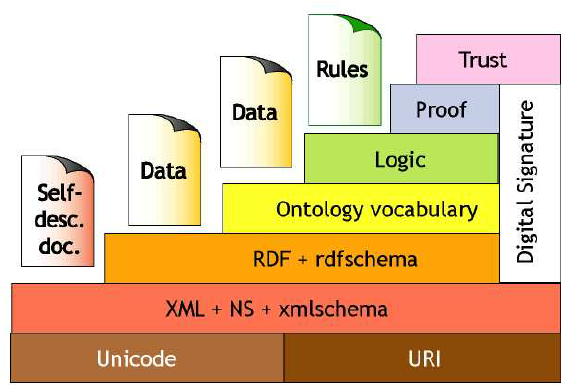
\includegraphics[width=0.63\textwidth]{layered_architecture.png} \label{fig:layered}
	\caption{Arhitectura stratificată pentru semantic web}
\end{figure}



\textbf{Caracteristici:}
\begin{itemize}
	\item SaaS business model
	\item Platformă software open source
	\item Personalizarea aplicațiilor pentru utilizatori
	\item Pooling de resurse
	\item Web inteligent
\end{itemize}


\textbf{Provocări:}
\begin{itemize}
	\item \emph{Vastitate} - conține miliarde de pagini, ce duce la redundanța datelor
	\item \emph{Vaguitatea} - interogările inprecise de către utilizatori, precum și modul în care furnizorii de conținut reprezintă conceptele pot face dificilă potrivirea termenilor de interogare cu termenii relevanți ai furnizorului. Acest lucru poate fi și mai agravat atunci când se încearcă integrarea mai multor baze de cunoștințe, care pot deține concepte similare, dar nu identice, ce poate rezulta în ambiguitate și incertitudine
	\item \emph{Incoerența} - contradicții logice ce vor apărea inevitabil
	\item \emph{Înșelăciune} - momentul în care sursa de informații induce în eroare intenționat consumatorul de informații
\end{itemize}

% \newpage
\section{Evolu\c tia tehnologiilor}

Pe măsură ce dezvoltarea aplicațiilor evolua, la fel au evoluat și tehnologiile utilizate în crearea aplicațiilor. De-a lungul anilor au apărut multe tehnologii care au revoluționat modul în care sunt dezvoltate aplicațiile. Pe măsură ce acestea deveneau mai complexe, necesitatea în tehnologii mai performante a devenit evidentă. La mijlocul anilor 2000 a fost introdus AJAX (\emph{Asynchronus JavaScript and XML}), care a permis aplicațiilor web să comunice cu serverele, fără a reîncărca întreaga pagină. Acest lucru a rezultat în aplicații web mai rapide și receptive.

În ultimii ani, au apărut mai multe framework-uri front-end, care au facilitat crearea aplicațiilor web cu o complexitate sporită. React, Vue, Next, Angular au devenit extrem de populare datorită ușurinței de utilizare și capacității lor de a gestiona cantități mari de date. Aceste framework-uri au făcut posibilă crearea unor aplicații cu un user experience și funcționalități ce nu au fost posibile anterior.

Pe lângă framework-urile front-end, au evoluat și tehnologiile back-end, în mod semnificativ. PHP, Ruby on Rails, Node.js au facilitat crearea aplicațiilor web moderne scalabile, care pot gestiona cantități mari de trafic în timp real și sarcini complexe de procesare a datelor.

Evoluția tehnologiilor web a fost determinată de necesitatea de a crea aplicații mai complexe, cu funcționalități avansate. De la HTML "curat" la framework-uri pentru front-end și back-end, tehnologiile web continuă să evolueze într-un ritm rapid, fapt ce impune dezvoltatorii să fie la curent cu ultimele tehnologii și constant să-și actualizeze metodele de dezvoltare utilizate, pentru a deveni mai efectivi în dezvoltarea aplicațiilor moderne, care răspund nevoilor sporite ale utilizatorilor.

\begin{figure}[htbp]
	\centering
	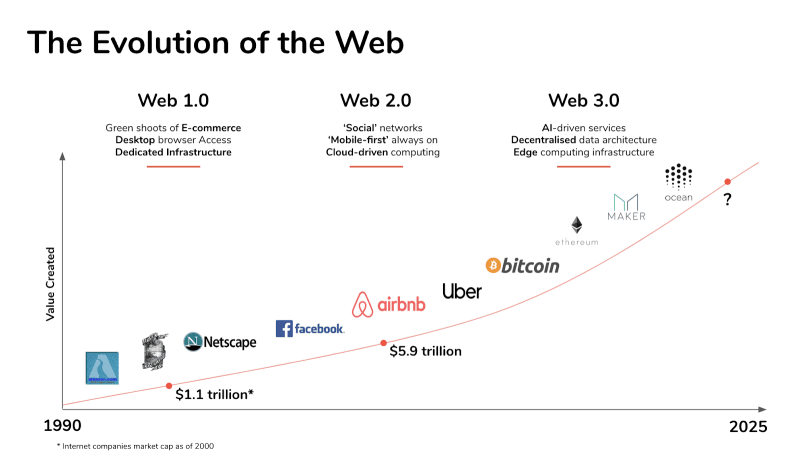
\includegraphics[width=0.9\textwidth]{web-evolution.png} \label{fig:web-evolution}
	\caption{Evolu\c tia web-ului}
\end{figure}

Evolutia web a avut un impact semnificativ asupra dezvoltării aplicațiilor web moderne. Creșterea vitezei de conectare la internet și a performanței dispozitivelor a permis dezvoltarea aplicațiilor web complexe, cu funcții avansate și user experience sporit. Utilizarea extinsa a standardelor web deschise, cum ar fi HTML, CSS și JavaScript, a dus la o mai mare interoperabilitate între diferite platforme și la o mai mare eficiență în dezvoltarea aplicațiilor.

Apariția și popularizarea API-urilor și a arhitecturilor RESTful au făcut posibilă integrarea mai ușoară a aplicatiilor web cu alte aplicații și servicii. Cloud computing-ul și serviciile web, cum ar fi Amazon Web Services și Microsoft Azure, au făcut posibilă scalabilitatea și distribuirea aplicațiilor web cu usurință, indiferent de locația utilizatorilor.

Creșterea numarului de utilizatori și a numarului de dispozitive conectate a dus la o creștere semnificativă a cerințelor de securitate și a necesității de a dezvolta aplicații web sigure.

Dezvoltarea și popularizarea framework-urilor și bibliotecilor de cod, cum ar fi Angular, React și Vue, a simplificat dezvoltarea aplicațiilor web și a îmbunatățit productivitatea dezvoltatorilor.

Aplicațiile web moderne sunt mult mai complexe și pot include o varietate de componente, cum ar fi front-end, back-end, baze de date, API-uri și multe altele. În plus, aplicațiile web trebuie să functioneze pe o varietate de platforme și dispozitive, ceea ce adaugă o altă dimensiune a complexității.

Pe masură ce aplicațiile web devin mai complexe, devin mai dificil de dezvoltat și de întreținut. Dezvolatorii trebuie să se concentreze nu numai pe funcționalitatea aplicației, ci și pe asigurarea securității și performanței acesteia. În plus, este necesar să se mențină un echilibru între user experience, securitate și scalabilitatea aplicației.

Pentru a face față acestei complexități, dezvoltatorii utilizează framework-uri și biblioteci care simplifică procesul de dezvoltare și permite o gestionare mai bună a complexității aplicațiilor.


\chapter{Paradigmele actuale de randare}
Rendering-ul este procesul de conversie a datelor într-o reprezentare vizuală și joacă un rol esențial în aplicațiile web, permițând furnizarea de conținut dinamic și interactiv către utilizatori.În stadiile incipiente ale dezvoltării web-ului, randarea a fost realizată în principal pe server. Site-urile web erau construite folosind tehnologii precum PHP sau Java, unde serverul genera conținutul HTML în mod dinamic, pe baza solicitărilor utilizatorilor. Această abordare are Time to first byte (TTFB) rapid, deoarece serverul poate genera HTML ce poate fi livrat rapid clientului. Dezavantajul acestei paradigme este c\u a nu este la fel de efectivă pentru site-urile web \^ in care datele se schimb\u a des, ci doar pentru site-urile care nu necesit\u a interactivitate complexă sau date dinamice. \cite{benefitsserverrendering}

Multe dintre cele mai mari aplica\c tii web din ziua de azi \^ inc\u a folosesc aceast\u a abordare, cum ar fi, de exemplu, amazon.com: de fiecare dat\u a c\^ and face\c ti click pe un link, ob\c tine\c ti o nou\u a pagin\u a generat\u a dinamic de pe serverele lor. \^ In plus, exist\u a multe framework-uri pentru crearea  aplica\c tiilor multi-page, cum ar fi Ruby on Rails, Django \c si Laravel, precum \c si sisteme de gestionare a con\c tinutului, cum ar fi WordPress. 

\section{Starea de art\u a}

Rendering-ul informa\c tiilor a evoluat semnificativ pe parcursul timpului, \^ in conformitate cu evolu\c tia tehnologiilor web \c si a cerin\c telor utilizatorilor.

La \^ inceput, majoritatea con\c tinutului era generat pe server \c si returnat c\u atre browser \^ in form\u a de pagini HTML statice. Cu trecerea timpului, tehnologiile web au evoluat, ceea ce a permis procesarea dinamic\u a a datelor în browser prin intermediul script-urilor. Acest lucru a permis dezvoltarea de aplica\c tii web cu interac\c tiuni complexe \c si randare dinamic\u a a con\c tinutului. Cu toate acestea, performan\c ta aplica\c tiilor web bazate exclusiv pe randare client-side a putut fi limitat\u a \^ in condi\c tii de conexiune lent\u a la internet. Din acest motiv, tehnologiile de randare hibrid\u a au devenit din ce \^ in ce mai populare, combin\^ and avantajele rand\u arii server-side \c si client-side. \cite{html}

\^ In prezent, tehnologiile de randare se bazeaz\u a pe framework-uri \c si biblioteci moderne, cum ar fi React, Angular \c si Vue, care ofer\u a unelte puternice pentru a construi aplica\c tii web performante \c si cu o experien\c t\u a utilizator remarcabil\u a. \^ In plus, tehnologiile de randare moderne permit integrarea cu alte tehnologii precum WebAssembly \c si Web Workers, care au ca scop \^ imbun\u at\u a\c tirea performan\c tei aplica\c tiilor web. De asemenea, tehnologiile de randare permit utilizarea de anima\c tii \c si interac\c tiuni complexe, care rezultă într-un user experience sporit al aplicației.

Evolu\c tia tehnologiei web \c si a cerin\c telor utilizatorilor continu\u a, iar randarea informa\c tiilor este un domeniu \^ in continu\u a schimbare \c si dezvoltare. \^ In etapa curent\u a de dezvoltare a aplica\c tiilor web, predomin\u a utilizarea larg\u a a JavaScript \c si bibliotecilor JavaScript, cum ar fi React \c si Vue.js.

React, dezvoltat de Facebook, a devenit una dintre tehnologiile cele mai populare pentru construirea de aplica\c tii web, datorit\u a abilit\u a\c tii sale de a oferi o experien\c t\u a de randare eficient\u a \c si de \^ inalt\u a performan\c t\u a. Vue.js, dezvoltat de comunitate, se concentreaz\u a pe simplitate \c si u\c surin\c t\u a de utilizare, fiind o alegere popular\u a pentru proiecte mai mici sau pentru dezvoltatorii care \^ incearc\u a s\u a \^ inve\c te tehnologii moderne de randare a informa\c tiilor.

Exist\u a mai multe tipuri de randare a con\c tinutului, cele mai populare fiind randarea \emph{server-side}, \emph{client-side} \c si  \emph{static server generation}: \cite{clientsidevssercerside}
\begin{enumerate}
	\item \textbf{Server-side rendering:} Procesarea datelor \c si generarea HTML se realizeaz\u a pe server. Server-ul returneaz\u a apoi HTML-ul generat c\u atre browser, care \^il afi\c seaz\u a utilizatorului. Aceast\u a metod\u a de randare este utilizat\u a \^in mod traditional \^in aplica\c tiile web vechi. Avantajul acestei metode este c\u a se poate efectua o procesare a datelor pe server \c si se poate oferi o experien\c t\u a utilizator consistent\u a chiar \c si \^in condi\c tii de conexiune lent\u a la internet. Afișarea inițială a paginii poate fi rapidă deoarece clientul nu trebuie să aștepte încărcarea sau executarea JavaScript-ului înainte de afișarea conținutului.
	\item \textbf{Client-side rendering:} Browser-ul prime\c ste date brute \c si le proceseaz\u a prin intermediul unui script (cum ar fi JavaScript) pentru a genera HTML. Aceast\u a metod\u a de randare permite o flexibilitate mai mare \^in prezentarea con\c tinutului \c si ofer\u a posibilitatea de a construi interac\c tiuni complexe cu utilizatorul, cum ar fi formulare dinamice \c si componente grafice interactive. Dezavantajul acestei metode este c\u a necesit\u a mai mult\u a putere de procesare a clientului \c si poate fi mai pu\c tin performant\u a \^in condi\c tii de conexiune lent\u a la internet, deoarece clientul trebuie să aștepte descărcarea scripturilor și a datelor necesare înainte de a randa pagina.
	\item \textbf{Static server generation:} Paginile web sunt pregenerate și randate în timpul procesului de build al aplicației, rezultând în fișiere HTML statice care pot fi furnizate către client fără a fi necesară procesarea la nivelul serverului. Cu SSG, conținutul rămâne static până la următorul build al aplicației.
\end{enumerate}

\^ In ceea ce prive\c ste performan\c ta, tehnologiile moderne de randare a informa\c tiilor au avansat mult \^ in optimizarea vitezei de randare \c si a eficien\c tei resurselor. Una dintre abord\u arile moderne de optimizare a performan\c tei este utilizarea \emph{"virtual DOM"} (Document Object Model), care se caracterizează printr-o rerandare eficientă doar a componentelor ce au suferit modificări.
\^ In plus, tehnologiile de randare moderne pot delimita componentele dinamice, care necesită rerandare constantă, de cele statice, care nu necesit\u a recalculare, cresc\^ and astfel performan\c ta aplica\c tiei. De asemenea, tehnologiile de randare permit utilizarea de tehnici de lazy loading, care \^ incarc\u a con\c tinutul doar atunci c\^ and este necesar, \^ imbun\u at\u a\c tind astfel performan\c ta aplica\c tiei \c si experiența utilizatorului.
Alegerea metodei potrivite de randare depinde de cerin\c tele specifice ale proiectului \c si poate include considera\c tii legate de performan\c ta, flexibilitatea \c si compatibilitatea cu echipamentele utilizatorilor. Este important s\u a se \^ in\c teleag\u a avantajele \c si dezavantajele fiec\u arei metode \c si s\u a se fac\u a o evaluare corespunz\u atoare a acestora \^ inainte de a lua o decizie.


\section{Client side rendering}

Re\^ inc\u arcarea \^ intregii pagini la fiecare schimbare de URL este un proces costisitor, de aceea pentru a reduce necesitatea de a regenera con\c tinutul au ap\u arut solu\c tii precum React \c si Angular - framework-uri JavaScript, ce permit modificarea componentelor f\u ar\u a a cauza o re\^ inc\u arcare a paginii. Aceast\u a arhitectur\u a se nume\c ste SPA (\textit{Single Page Application}).

Într-un SPA, resursele HTML, CSS și JavaScript inițiale sunt încărcate atunci când aplicația este accesată pentru prima dată. Interacțiunile ulterioare și modificările stării aplicației sunt gestionate prin efectuarea de cereri asincrone către server pentru a obține date, care sunt apoi randate pe partea de client (\textit{client-side rendering}). Aceasta rezultă \^intr-o experiență mai receptivă și interactivă, deoarece aplicația poate actualiza componente sau secțiuni specifice ale paginii fără a comunica cu serverul.

O aplica\c tie ce utilizeaz\u a CSR este caracterizat\u a prin urm\u atoarele aspecte:
\begin{enumerate}
	\item \textbf{Cererea HTTP a clientului} - când utilizatorul introduce URL-ul în bara de adrese a browserului, se stabilește o conexiune HTTP cu serverul.
	\item \textbf{Răspunsul HTTP al serverului} - Serverul trimite înapoi fișierul HTML inițial, care conține referințe către fișiere JavaScript și CSS.
	\item \textbf{Încărcarea paginii} - browserul clientului primește fișierul HTML inițial și începe randarea structurii de bază a paginii, inclusiv orice conținut static.
	\item \textbf{Încărcarea fișierelor JavaScript} - browserul descarcă fișierele JavaScript referen\c tiate în fișierul HTML inițial.
	\item \textbf{Preluarea datelor} - codul JavaScript executat de browserul clientului face cereri către server sau API-uri, pentru a prelua datele necesare pentru a randa conținutul dinamic.
	\item \textbf{Randarea \c si actualizarea} - odată ce datele sunt preluate, codul JavaScript procesează datele și generează dinamic structura HTML necesară. Browserul actualizează pagina randat\u a cu conținutul HTML generat dinamic, care poate include liste, tabele, formulare sau alte componente
	\item \textbf{Interactivitatea} - ascultătorii de evenimente și interacțiunile utilizatorului, cum ar fi click-urile sau introducerile de date, declanșează execuția de cod JavaScript ulterioară, care poate actualiza conținutul randat, fără a necesita o reîncărcare completă a paginii.
\end{enumerate}

\begin{figure}[htbp]
	\centering
	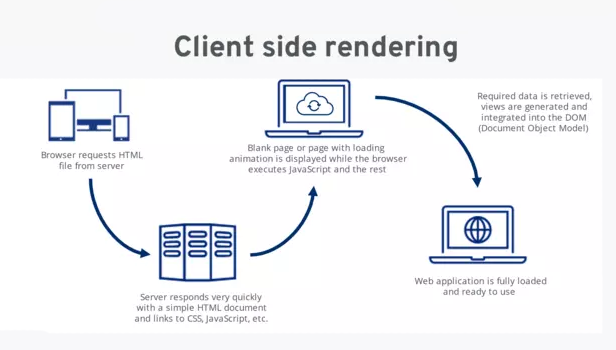
\includegraphics[width=0.9\textwidth]{csr-diagram.png}
	\caption{Client side rendering}
	\label{fig:csr-diagram}
\end{figure}

Deoarece browserul trebuie să descarce și să ruleze întregul cod al aplicației înainte ca conținutul să apară pe ecran, încărcarea inițială a paginii este de obicei lentă. Ca rezultat, utilizatorii văd o pagină goală sau un indicator de încărcare pentru o perioadă relativ lungă de timp. Aceasta duce la o experiență mai puțin plăcută pentru utilizatori și la o rată mai mare de abandon\u ari a paginii (\textit{bounce rate}). \cite{google-bouncing-rate}

Cu toate acestea, pot exista provocări în ceea ce privește optimizarea pentru motoarele de căutare (SEO), deoarece toate resursele aplicației sunt \^inc\u arcate la prima accesare, crawler-ii web tradiționali pot întâmpina dificultăți în parcurgerea și indexarea conținutului, iar volumul mare de scripturi ce sunt descărcate, bibliotecile externe \c si dependențele pot rezulta \^intr-un timp de încărcare inițial mai mare.

\section{Server side rendering}

O nou\u a abordare, ce avea scopul de a rezolva problemele aplicatiilor single page este server-side rendering (SSR).

SSR este o tehnică în dezvoltarea aplicațiilor web care implică generarea de HTML pe server și trimiterea acestuia către client. Spre deosebire de CSR, procesul de randare se execut\u a pe server, ce reprezintă un avantaj semnificativ, datorită timpului mai rapid de încărcare inițială a paginilor. \cite{benefitsserverrendering}

\begin{figure}[htbp]
	\centering
	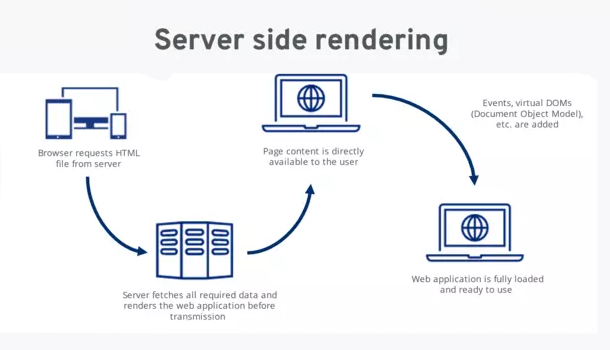
\includegraphics[width=0.9\textwidth]{ssr-diagram.png}
	\caption{Server side rendering}
	\label{fig:ssr-diagram}
\end{figure}

Un alt avantaj al SSR este îmbunătățirea optimizării pentru motoarele de căutare (SEO). Deoarece crawler-ii motoarelor de căutare se bazează în mod tipic pe conținutul HTML, serve-side rendering furnizează pagini complet randate motoarelor de căutare, care pot fi indexate ușor. Aceasta îmbunătățește vizibilitatea și accesibilitatea site-ului în rezultatele motoarelor de căutare.

SSR aduce beneficii și utilizatorilor cu conexiuni lente la internet sau dispozitive mai vechi. Prin pre-randarea HTML-ului pe server, SSR asigură utilizatorii cu conținut chiar și în cazul în care dispozitivele lor au putere de procesare limitată sau capacități de rețea reduse. Aceasta îmbunătățește accesibilitatea și experiența utilizatorului pentru o gamă mai largă de utilizatori.

Server-side rendering are c\^ateva dezavantaje asociate. Deoarece fiecare solicitare necesită o nouă randare pe server, aceasta poate duce la o încărcare mai mare a serverului și la un timp de răspuns mai lent. De asemenea, este mai dificil de implementat și de întreținut, deoarece necesită o infrastructură de servere mai complexă. SSR creează o dependență de server, deoarece clientul primește pagini complet redată de la server. În cazul în care serverul întâmpină probleme sau este indisponibil, utilizatorii nu pot accesa sau utiliza aplicația.
Gestionarea stării clientului poate deveni și mai complexă cu SSR. Sincronizarea și actualizarea stării între client și server pentru a menține coerența aplicației necesită o implementare bine gândită și poate fi dificil de gestionat.

O aplicație ce utilizează SSR este caracterizat\u a prin următoarele aspecte:

\begin{enumerate}
	\item \textbf{Cererea HTTP din partea clientului} - c\^and utlizitorul introduce URL-ul \^in broswer, se stabile\c ste o conexiune HTTP cu serverul \c si apoi se trimite serverului o cerere pentru a ob\c tine documentul HTML.
	\item \textbf{Preluarea datelor} - serverul preia datele necesare din baza de date sau API-uri.
	\item \textbf{Pre-randarea pe partea de server} - serverul compileaz\u a componentele JavaScript \^in HTML static.
	\item \textbf{Răspunsul HTTP al serverului} - serverul trimite documentul compilat c\u atre client.
	\item \textbf{Încărcarea și afișarea paginii} - clientul descarc\u a fi\c sierul HTML \c si afi\c seaz\u a componentele statice pe pagină.
	\item \textbf{Hidratarea} - clientul descarcă fișierul sau fișierele JavaScript încorporate în HTML, procesează codul și atașează ascultători de evenimente componentelor.
\end{enumerate} \cite{improve-ssr-speed}

\section{Static server generation}

SSG este o paradigma alternativă în dezvoltarea web care îmbină beneficiile SSR și CSR. Spre deosebire de server-side rendering, unde HTML-ul este generat dinamic la fiecare cerere, SSG generează fișiere HTML statice în timpul procesului de build, care sunt apoi servite către client.

\begin{figure}[htbp]
	\centering
	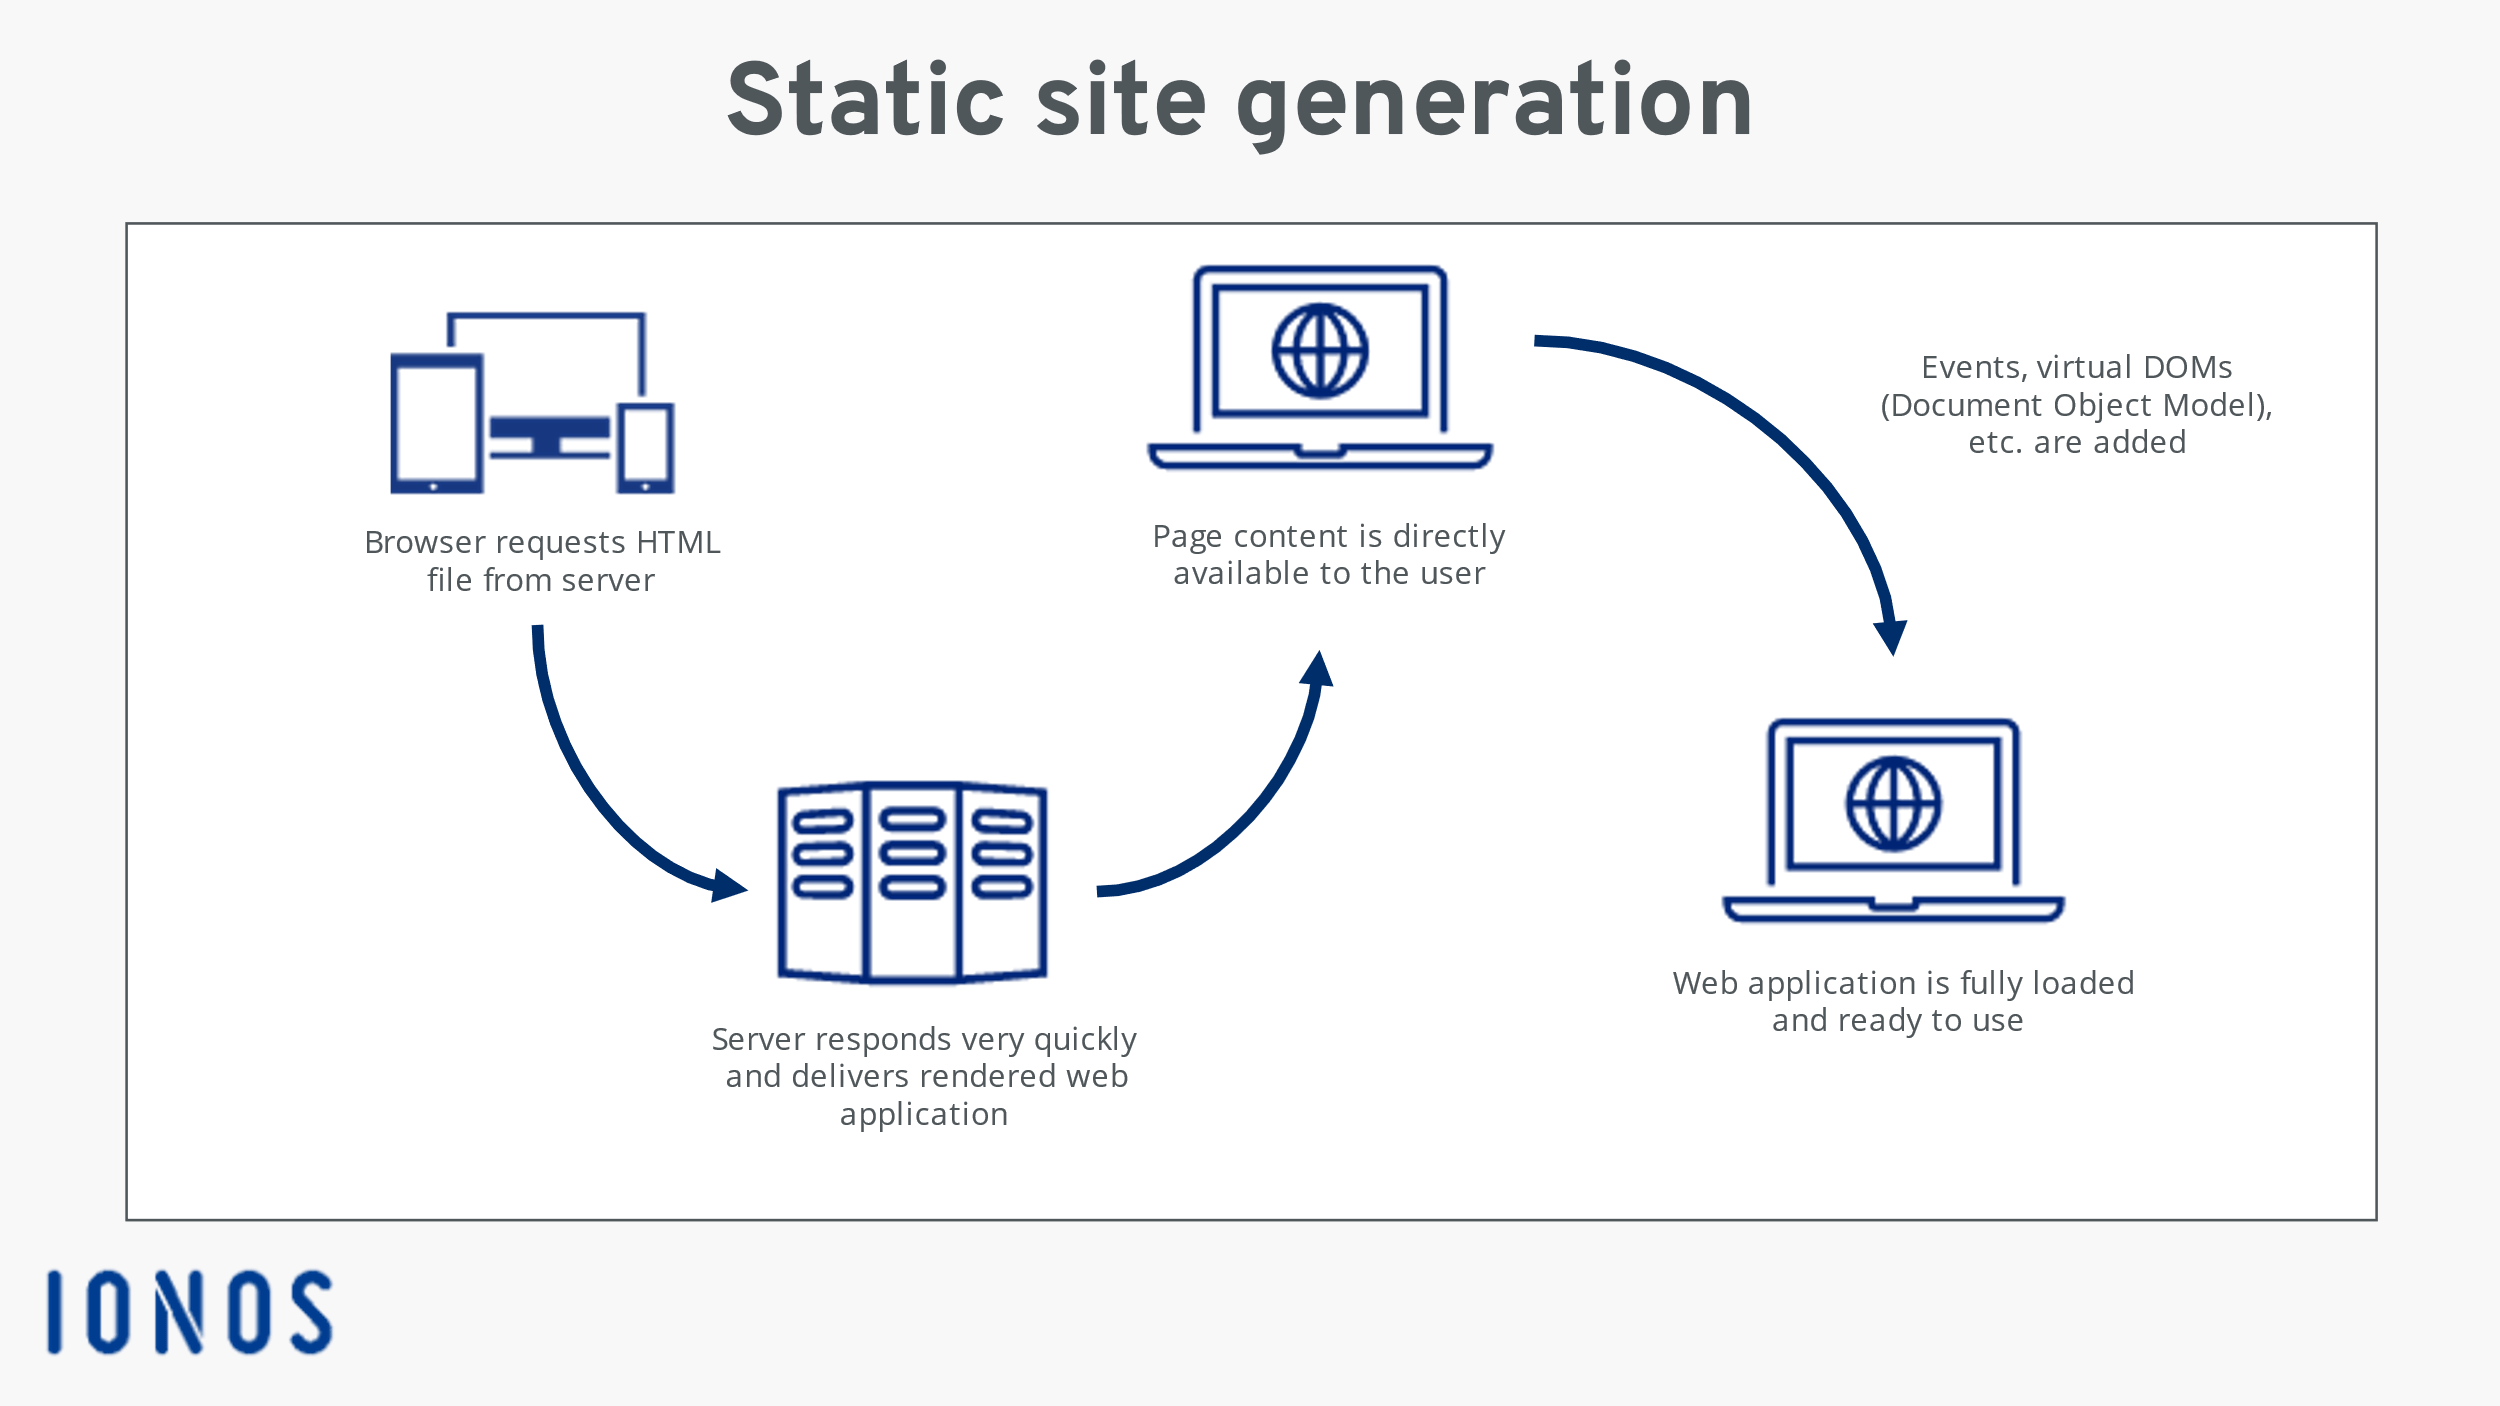
\includegraphics[width=0.8\textwidth]{ssg-diagram.png}
	\caption{Static server generation}
	\label{fig:ssg}
\end{figure}

Unul dintre avantajele majore ale SSG este performanța îmbunătățită și scalabilitatea. Deoarece HTML-ul este pre-randat, serverul poate servi fișiere statice direct, fără a necesita prelucrări suplimentare. Aceasta duce la încărcarea mai rapidă a paginilor și reducerea încărcării serverului, făcându-l potrivit pentru site-urile cu trafic intens. 

O aplicație ce utilizează SSR este caracterizat\u a prin următoarele aspecte:
\begin{enumerate}
	\item \textbf{Procesul de build} - \^in timpul acestui proces codul sursă și fișierele de conținut ale site-ului web sunt analizate.
	\item \textbf{Compilarea conținutului} - con\c tinutul fi\c sierelor este procesat \c si convertit din formatul sursă (Markdown sau YAML) în formatul HTML.
	\item \textbf{Modelarea} - sunt aplicate \c sabloane pe fi\c sierele compilate, permițând un aspect și o structură coerent\u a.
	\item \textbf{Integrarea datelor} - sunt preluate date din diverse surse (baze de date, API-uri) \c si sunt integrate în paginile generate anterior.
	\item \textbf{Generarea HTML-ului static} - fi\c sierele HTML sunt generate pe baza con\c tinutului compilat, a \c sabloanelor \c si a datelor integrate.
	\item \textbf{Optimizarea resurselor} - \^in timpul procesului de build, resursele precum CSS, JavaScript și imaginile se optimizeaz\u a, reducând dimensiunile fișierelor și îmbunătățind performanța.
	\item \textbf{Implementarea} -  odată ce fișierele statice sunt generate, acestea pot fi păstrate în cache pe server sau pe CDN, permițând servirea instantanee a cererilor ulterioare fără a necesita regenerarea lor (\textit{minimizează încărcarea serverului și îmbunătățește scalabilitatea generală, în special în scenarii în care actualizările de conținut sunt rare}).
	\item \textbf{Cererea clientului} -  când un utilizator vizitează o pagină, serverul web sau CDN-ul servește direct fișierul HTML static pre-generat.
	\item \textbf{Afișarea paginii} - browserul clientului primește fișierul HTML static și afișează conținutul pe pagină.
	\item \textbf{Interactivitatea} - Dacă există elemente interactive sau funcționalități dinamice pe pagină, codul JavaScript poate fi utilizat pentru a îmbunătăți experiența utilizatorului, de obicei prin preluarea de date suplimentare din API-uri sau prin gestionarea interacțiunilor utilizatorului.
\end{enumerate}

Cu toate acestea are și câteva limitări. SSG nu este potrivit pentru aplicații ce necesită actualizări în timp real sau conținut dinamic, deoarece fișierele statice pre-randate nu se modifică până la următorul proces de build. Acest lucru poate introduce întârzieri în disponibilitatea conținutului și creșterea complexității gestionării actualizărilor de conținut.
Unul dintre cele mai mari dezavantaje ale acestui abordări este timpul de build. Dacă site-ul cons\u a dintr-un num\u ar mare de pagini, procesul de build al acestora va dura mult timp.


\section{Alegerea paradigmei corespunzătoare}

Alegerea între CSR, SSR și SSG este importantă în dezvoltarea unei aplicații web, deoarece are un impact direct asupra experienței utilizatorului, performanței și funcționalit\u a\c tii generale a aplicației. Fiecare abordare are propriile sale puncte forte și considerații, iar alegerea depinde de mai mul\c ti factori, cum ar fi cerințele proiectului, scalabilitatea, complexitatea și obiectivele de performanță. Principalele aspecte de luat în considerare sunt:

\begin{enumerate}
	\item \textbf{Experiența utilizatorului} - Abordarea de randare afectează în mod semnificativ modul în care conținutul aplicației este livrat în browserul utilizatorului. CSR pune accent pe interactivitate, prin încărcarea inițială a unei structuri HTML minimale și apoi preluarea și randarea datelor pe partea clientului, ceea ce duce la o încărcare inițială mai rapidă a paginii. SSR, pe de altă parte, furnizează o pagină HTML complet redată de pe server, fapt ce reduce timpul de încărcare inițial și asigur\u a ca conținutul să fie imediat vizibil utilizatorilor. SSG generează fișiere HTML statice în timpul procesului de construcție, permitând încărcări de pagini ultra-rapide, deoarece nu este necesară prelucrarea în server.
	\item \textbf{Optimizarea pentru motoarele de căutare} - Motoarele de căutare întâmpină adesea dificultăți în indexarea conținutului JavaScript dinamic. SSR și SSG, care livrează conținut HTML pre-randat în browser, sunt mai efective cu SEO în comparație cu CSR. Acest lucru se datorează faptului că motoarele de căutare pot parcurge și indexa ușor conținutul HTML static, ceea ce ajută la îmbunătățirea vizibilității și descoperirii.
	\item \textbf{Performanța} - Abordarea de randare afectează performanța generală a aplicației. CSR poate duce la timp de încărcare mai lung, în special în cazul conexiunilor de rețea mai lente sau al unor cantități mari de date de preluat. SSR reduce timpul de randare inițial prin furnizarea unei pagini pre-randate de pe server, \^ins\u a navigarea ulterioară poate necesita apeluri suplimentare către server. SSG oferă cea mai bună performanță, deoarece generează fișiere HTML statice care pot fi livrate direct utilizatorului, minimizând necesitatea de prelucrare pe server.
	\item \textbf{Complexitatea și fluxul de dezvoltare} - Framework-urile CSR, cum ar fi React, Angular sau Vue.js, necesită ca dezvoltatorii să gestioneze logica de randare și stăriile componentelor, ceea ce poate introduce complexitate. SSR și SSG reduc, într-o anumită măsură, această complexitate prin transferul logicii de randare la server sau la procesul de build al aplicației. SSR necesită configurare pe partea de server și cunoștințe despre tehnologiile backend, în timp ce SSG simplifică fluxul de lucru în dezvoltare prin generarea de active statice care pot fi ușor implementate pe orice server web.
	\item \textbf{Conținutul dinamic și actualizări în timp real} - CSR se evidențiază în aplicațiile extrem de interactive care se bazează pe actualizări frecvente ale datelor sau pe funcționalități în timp real. Cu CSR, datele pot fi actualizate fără necesitatea unei re\^inc\u arc\u ari complete a paginii. SSR și SSG sunt mai potrivite pentru aplicațiile axate pe conținut mai puțin dinamic, deoarece necesită o solicitare către server pentru a actualiza datele.
\end{enumerate}

Alegerea paradigmei potrivite este esențială pentru a furniza o aplicație web rapidă, interactivă și optimizat\u a pentru motoarele de c\u autare. De asemenea, este important să se ia în considerare cerințele proiectului, complexitatea și obiectivele de performanță pentru a determina cea mai bună abordare de randare. Aceasta este una dintre primele decizii importante ce trebuie luat\u a în dezvoltarea unei aplicații web, deoarece este dificil de schimbat ulterior.

\chapter{Aplicația practică}

Obiectivul acestui capitol este de a oferi o experiență practică cu tehnologiile de randare și de a evalua performanța și eficiența acestora. Rezultatele obținute vor fi valoroase pentru dezvoltatori și arhitecți care doresc să optimizeze procesele de randare și să îmbunătățească experiența utilizatorului.

% Pentru obiectivitatea experimentului, a fost implementa aceeași aplicație cu ajutorul la mai multe framework-uri JavaScript, cât și în vanilla (\emph{plain}) JavaScript, pentru a obține rezultate ce se vor putea compara, pentru a identifica cele mai optime abordari posibile.

Pentru o obiectivitate sporită a fost implementată aceea\c si aplica\c tie, cu ajutorul mai multor framework-uri JavaScript, fiecare dintre ele reprezent\^and o abordare diferit\u a de randare (CSR, SSR, SSG). De asemenea, aplicația a fost implementat\u a \c si cu ajutorul vanilla JavaScript, pentru a compara aplicațiile dup\u a un anumit set de criterii cu scopul de a identifica care sunt aspectele cheie care diferă între aplicațiile construite cu ajutorul framework-urilor JavaScript și cea construită folosind vanilla JavaScript. Rezultatul acestui studiu comparativ ofer\u a o imagine de ansamblu asupra avantajelor și dezavantajelor fiecărei tehnici de randare, precum și a celor mai optime abordări posibile.


\section{Metrici de performanță}

Pentru compararea efectivă a metodelor de implementare, este nevoie de a compara rezultatele după anumite criterii care reprezintă performanța generală a aplicației.

Metricile care vor fi utilizate în evaluarea performanței pentru toate implementările sunt:

\begin{itemize}
	\item \textbf{Largest Contentful Paint (\emph{LCP})} - metrică de performanță utilizată pentru a măsura viteza de încărcare și stabilitatea vizuală percepută a unei pagini web, introdusă de Google. LCP măsoară timpul necesar ca cel mai mare element vizibil de pe o pagină web să fie afișat în zona de vizualizare a utilizatorului. Acest element poate fi o imagine, un videoclip sau un element de tip block, cum ar fi un paragraf sau un antet. Cu cât LCP este mai rapid, cu atât este mai bună experiența utilizatorului, deoarece indică faptul că conținutul principal al paginii este afișat rapid. Un scor bun al LCP este considerat în general sub 2,5 secunde. Dacă LCP depășește acest prag, poate duce la o rată mai mare de respingere și poate afecta negativ angajamentul utilizatorului. Pentru a îmbunătăți LCP, dezvoltatorii web pot optimiza performanța site-ului prin minimizarea resurselor care blochează afișarea, optimizarea imaginilor și videoclipurilor și implementarea tehnicilor precum lazy-load și code splitting.

	      LCP este una dintre principalele metrici luate în considerare de motoarele de căutare, inclusiv Google, pentru a evalua experiența utilizatorului pe un site web. Site-urile cu scoruri bune ale LCP sunt mai susceptibile de a obține un rang mai înalt în rezultatele căutării și de a oferi o experiență de navigare mai bună utilizatorilor.
	\item \textbf{Cumulative Layout Shift (\emph{CLS})} - este utilizată pentru a măsura stabilitatea vizuală a unei pagini web. Aceasta cuantifică cantitatea de schimbări de aspect neașteptate care apar în timpul încărcării paginii. Schimbarea de aspect se referă la mișcarea elementelor paginii, cum ar fi imagini, butoane sau text, într-un mod care perturbă experiența de citire sau de interacțiune a utilizatorului. Aceste schimbări pot fi frustrante pentru utilizatori, în special atunci când cauzează click-uri accidentale sau fac conținutul dificil de citit.

	      CLS este calculat prin măsurarea frac\c tiunii de impact și frac\c tiunii de distanță a fiecărui eveniment de schimbare de aspect și apoi însumându-le pe întreaga încărcare a paginii. Frac\c tiunea de impact reprezintă proporția vizualizării afectată de schimbare, în timp ce frac\c tiunea de distanță reprezintă distanța maximă pe care elementul o parcurge în raport cu ecranul utilizatorului.

	      Pentru a oferi o bună experiență utilizatorului, o pagină web ar trebui să aibă un scor CLS scăzut. Un scor CLS sub 0.1 este considerat excelent, între 0.1 și 0.25 este considerat bun, în timp ce scorurile peste 0.25 sunt considerate slabe.

	      Pentru a reduce CLS, dezvoltatorii web pot urma practici, cum ar fi stabilirea dimensiunilor explicite pentru elementele media, rezervarea spațiului pentru reclame sau conținut dinamic și evitarea injectării dinamice a conținutului deasupra elementelor existente. Prin minimizarea schimbărilor de aspect neașteptate, dezvoltatorii pot îmbunătăți stabilitatea vizuală a paginilor web și experiența utilizatorilor.
	\item \textbf{First Input Delay (\emph{FID})} - măsoară reactivitatea și interactivitatea unei pagini web. Ea cuantifică timpul necesar ca o pagină web să răspundă la prima interacțiune a utilizatorului, cum ar fi apăsarea unui buton sau selectarea unui meniu derulant.

	      FID se concentrează în mod specific pe întârzierea dintre prima interacțiune a utilizatorului și capacitatea browserului de a răspunde la acea interacțiune. Este importantă deoarece reflectă reactivitatea percepută a unui site web și are un impact direct asupra experienței utilizatorului. Un FID redus indică un site web mai interactiv și mai receptiv, în timp ce un FID ridicat poate face un site web să pară lent și neinteractiv.

	      FID-ul este măsurat în milisecunde (ms), iar un scor bun este considerat a fi mai mic de 100 de milisecunde. Un scor peste 300 de milisecunde este considerat slab și poate rezulta într-o experiență frustrantă pentru utilizatori.

	      Pentru a îmbunătăți FID, dezvoltatorii web pot optimiza codul lor, reduce timpul de execuție al JavaScript-ului și prioritiza sarcinile critice pentru a asigura timp de răspuns mai rapid la interacțiunile utilizatorului. Tehnici precum minimizarea codului, împărțirea codului și încărcarea asincronă a scripturilor pot contribui la reducerea impactului JavaScript-ului asupra FID-ului.

	      FID-ul este una dintre metricile centrale ale aspectelor vitale ale webului utilizate de motoarele de căutare, inclusiv Google, pentru a evalua experiența utilizatorului pe un site web. Site-urile cu scoruri bune de FID au mai multe șanse să obțină un rang mai înalt în rezultatele căutării și să ofere o experiență de navigare mai fluidă și mai captivantă utilizatorilor.
	\item \textbf{Interaction to Next Paint (\emph{INP})} -  metrică a Core Web Vitals, care va înlocui First Input Delay (FID) din martie 2024. INP evaluează reactivitatea folosind date din Event Timing API. Atunci când o interacțiune determină ca o pagină să devină neproductivă, aceasta reprezintă o experiență utilizator slabă. INP observă latența tuturor interacțiunilor pe care le-a realizat utilizatorul cu pagina și raportează o valoare unică sub care au fost toate (sau aproape toate) interacțiunile. Un INP scăzut înseamnă că pagina a putut răspunde în mod constant și rapid tuturor sau unei mari majorități a interacțiunilor utilizatorului.

	      Unele interacțiuni vor dura mai mult decât altele, dar în special pentru interacțiunile complexe, este important să prezentați un feedback vizual inițial ca indiciu pentru utilizator că se întâmplă ceva în background. Timpul până la următoarea desenare (\emph{paint}) este cea mai timpurie oportunitate pentru a face acest lucru. Prin urmare, intenția INP nu este de a măsura toate efectele ulterioare ale interacțiunii (cum ar fi fetch-urile și actualizările UI din alte operații asincrone), ci timpul în care următoarea desenare este blocată. Prin întârzierea feedbackului vizual, puteți da utilizatorilor impresia că pagina nu răspunde acțiunilor lor.

	      Scopul INP este de a asigura ca timpul de la inițierea unei interacțiuni de către utilizator până la următoarea cadru desenat să fie cât mai scurt posibil, pentru toate sau majoritatea interacțiunilor realizate de utilizator.
\end{itemize}

\section{Metode de evaluare a performanței}

Există mai multe metode disponibile pentru măsurarea performanței unei aplicații web. Aceste instrumente pot ajuta dezvoltatorii să monitorizeze și să îmbunătățească performanța și experiența utilizatorilor.

În evaluarea aplicației curente au fost folosite următoarele metode de evaluare a performanței:

\begin{itemize}
	\item  \textbf{Web Vitals} (extensie pentru browser) - inițiativă de la Google care oferă ghidare unitară pentru semnalele de calitate care sunt esențiale pentru a oferi o experiență excelentă utilizatorilor pe web.

	      Google a furnizat de-a lungul anilor o serie de instrumente pentru a măsura și raporta performanța. Unii dezvoltatori sunt experți în utilizarea acestor instrumente, în timp ce alții au considerat că abundanța atât a instrumentelor, cât și a metricilor este dificilă de urmărit.  Inițiativa Web Vitals își propune să simplifice peisajul și să ajute site-urile să se concentreze pe metricile care contează cel mai mult, Core Web Vitals. Fiecare dintre Core Web Vitals reprezintă o componentă distinctă a experienței utilizatorului, este măsurabilă în teren și reflectă experiența reală a unui rezultat critic centrat pe utilizator.

	      Setul actual se concentrează pe trei aspecte ale experienței utilizatorului - încărcare, interactivitate și stabilitate vizuală - și include următoarele metrici: Largest Contentful Paint (LCP), First Input Delay (FID), Cumulative Layout Shift (CLS).

	\item \textbf{Lighthouse} chrome developer tool - unealtă de testare automată open-source dezvoltată de Google, care ajută la măsurarea și îmbunătățirea calității și performanței paginilor web. Aceasta oferă o analiză cuprinzătoare a diferitelor aspecte ale unei pagini web precum performanța, accesibilitatea, optimizare pentru motoarele de căutare (SEO) și altele. Lighthouse este folosit în mod frecvent de dezvoltatori pentru optimizarea site-urilor și aplicațiilor web în vederea obținerii unei experiențe mai bune pentru utilizatori.

	\item \textbf{PageSpeed Insights} website - unealtă de analiză a performanței web dezvoltată de Google. Aceasta oferă informații și recomandări pentru optimizarea vitezei și performanței unei pagini web. Prin analizarea conținutului unei adrese URL, PageSpeed Insights generează un raport care identifică probleme legate de performanță și sugerează îmbunătățiri.
\end{itemize}

\section{Compara\c tia \c si analiza practică a aplica\c tiilor}

Pentru a compara performanța dintre mai multe framework-uri JavaScript, este nevoie de o aplicație care va fi implementată în toate framework-urile, cu cât mai puține elemente distincte, pentru o evaluare cât mai obiectivă. Scopul acestei analize este de a determina care abordare oferă cea mai bună performanță în ceea ce privește timpul de încărcare al paginii, viteza de randare și experiența generală a utilizatorului. Totodată se vor lua în considerare ușurința implementării, documentația disponibilă și scalabilitatea efectivă a aplicației.

\subsection{Metodologie}

Pentru această comparație a performanței, am selectat vanilla JavaScript și React, datorită popularității și utilizării extinse. Am creat o aplicație demonstrativă care include o imagine de fundal aleatorie preluată de la un API extern, o listă de utilizatori și postări asociate preluate de pe un alt API, elemente ce conțin animații și stilizare a componentelor, un input care permite filtrarea utilizatorilor.

Performanța aplicației a fost testată atât în mediul local, cât și după deploy pe web hosting.

\subsection{Vanilla JavaScript}
Structura aplicație constă din trei fișiere:
\begin{itemize}
	\item \textbf{index.html} - conține markup-ul aplicației
	\item \textbf{app.js} - conține toată logica aplicației (data fetching, data rendering, data mutations)
	\item \textbf{style.css} - conține stilizarea elementelor html
\end{itemize}

\begin{figure}[htbp]
	\centering
	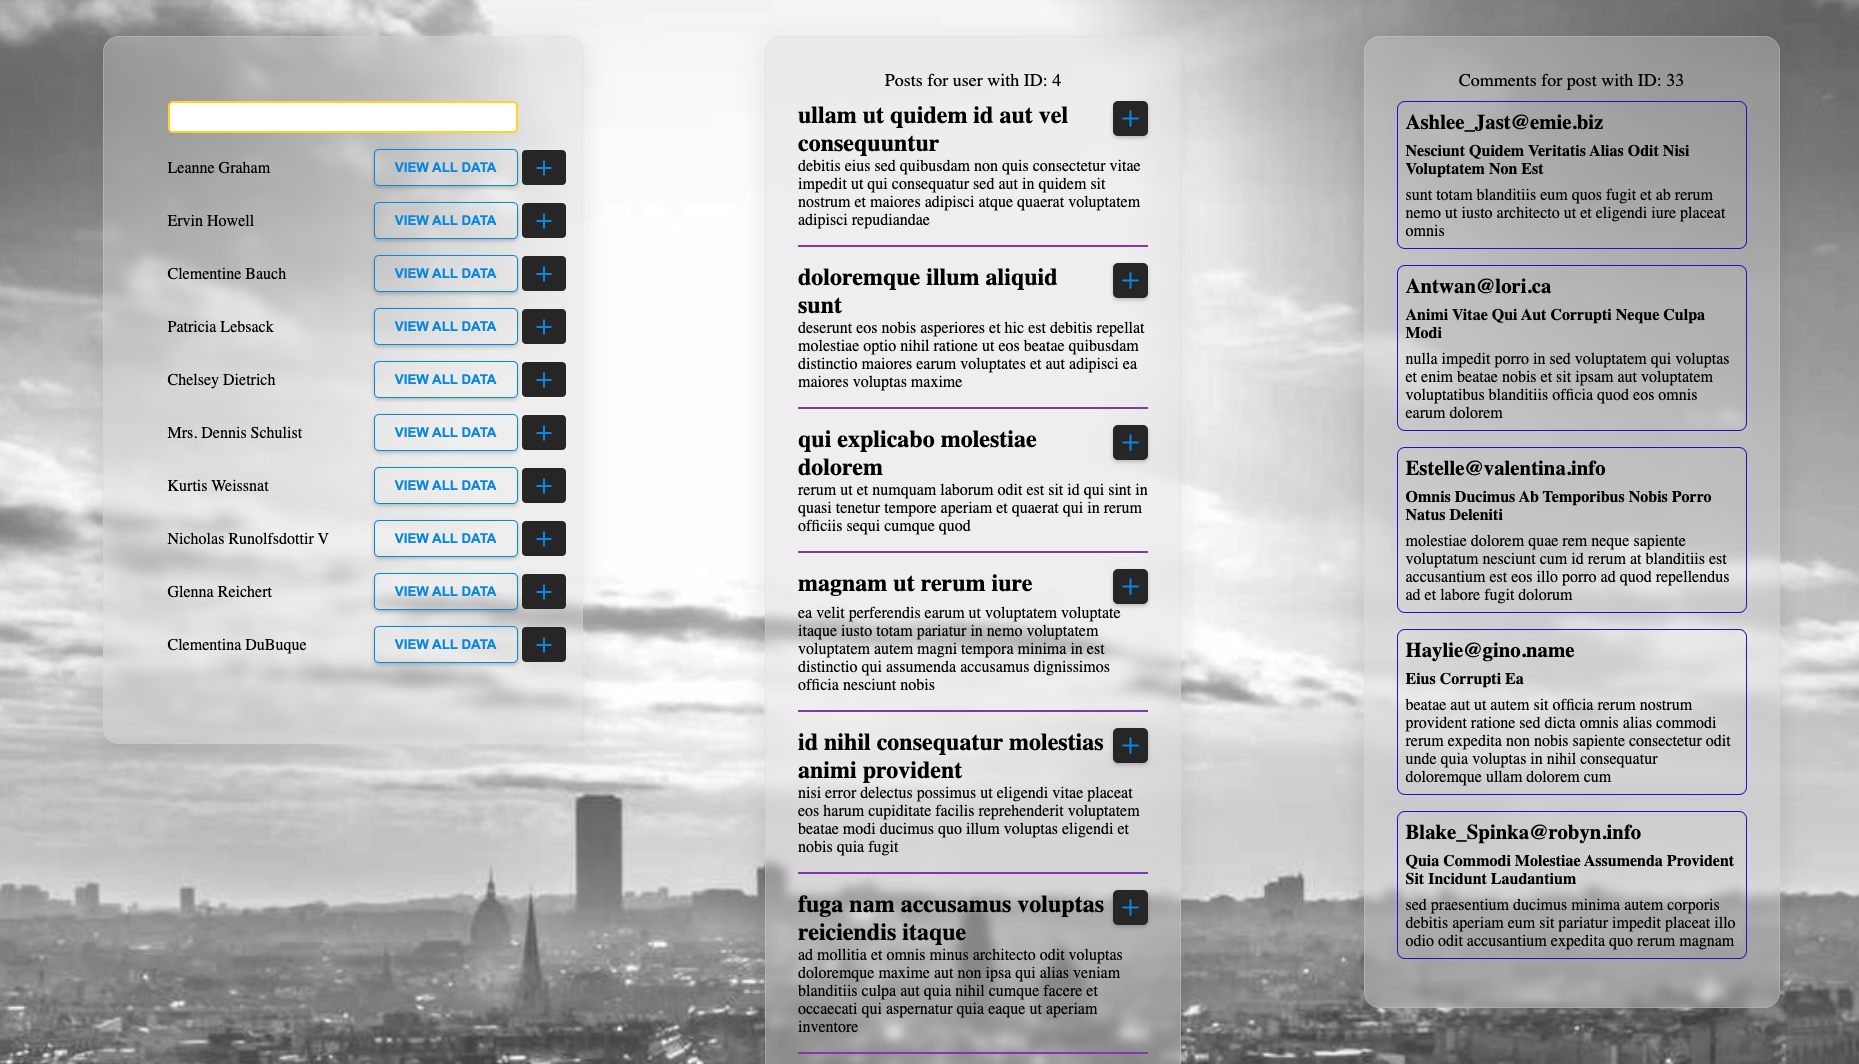
\includegraphics[width=0.9\textwidth]{01_desktop_preview.png}
	\caption{Aplicația practic\u a - vanilla JavaScript}
	\label{fig:preview-vanillajs}
\end{figure}

Pentru a obține datele de la API, am utilizat funcția  \emph{fetch}:
\begin{lstlisting}
	const usersRes = await fetch("https://jsonplaceholder.typicode.com/users");
	const postsRes = await fetch("https://jsonplaceholder.typicode.com/posts");
\end{lstlisting}

Pentru a implementa funcționalitatea de afișare a posturilor asociate unui utilizator, am utilizat localstorage pentru a stoca Id-ul și numele utilizatorului curent, pentru a folosi aceste date în funția de filtrare a posturilor
\begin{lstlisting}
	function handleSaveButtonClick(event) {
		localStorage.setItem("selectedUser", JSON.stringify(selectedUser));
	}

	async function renderPosts(data) {
		const postsUl = document.getElementById("posts");
		const selectedName = localStorage.getItem("selectedName");
  		const selectedUser = ALL_USERS.find((user) => user.name === selectedName);

		const html = data.map( (posts) => 
			`<li class="list-item-post"> 
			<h2 class='post-header'> ${post.title} </h2>
			<p> ${post.body} </p>
			</li>`).join("");

	  	postsUl.innerHTML += html;
	}

\end{lstlisting}
\subsection{React framework}

Cu ajutorul comenzii \emph{npx create-react-app 02-react} se generează un proiect React, cu numele 02-react, care va conține fișierele configurate și folderele necesare pentru aplicația React, inclusiv structura de bază a proiectului, fișierele de configurare implicite și dependențele inițiale.

\begin{figure}[htbp]
	\centering
	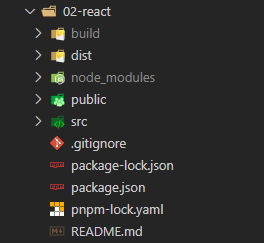
\includegraphics[width=0.4\textwidth]{react_file_structure.png}
	\caption{Strctura unei aplicații React}
	\label{fig:react-structure}
\end{figure}

Directorul "src" dintr-un proiect conține fișierele de cod sursă pentru aplicația React. Aici sunt scrise și organizate componentele, stilurile și alte fișiere relevante ale aplicației.

Aplicația construită cu React are câteva avantaje față de o aplicație construită cu plain JavaScript:

\begin{enumerate}
	\item \textbf{Eficiență și Performanță}: utilizarea Virtual DOM și a algoritmi eficienți de reconciliere pentru a actualiza și afișa doar componentele care s-au schimbat în loc de rerandarea întregului DOM. Acest lucru duce la o performanță mai bună și la o aplicație mai eficientă, în special în cazul aplicațiilor cu interfețe complexe și cu multe date.
	\item \textbf{Abordare declarativă}: React utilizează o abordare în care se definește starea dorită a interfeței utilizator și React se ocupă de actualizarea și afișarea acesteia în mod automat. Aceasta face codul mai ușor de înțeles și de gestionat, și reduce riscul de erori.
	\item \textbf{React hooks}:  funcții speciale furnizate de React, care permit componentelor funcționale să acceseze funcționalități specifice și să gestioneze logica acestora.
\end{enumerate}

Pentru a reține anumite date, precum utilizatorul curent, masivul de postări sau valoarea curentă a input-ului putem utiliza hook-ul \emph{useState}, ce permite gestionarea și actualizarea stării interne a unei componente, iar pentru a obține listele de utilizatori și postrări într-un mod efectiv, utilizăm hook-ul \emph{useEffect} pentru a ne asigura că acestea sunt executate la momentele potrivite în timpul ciclului de viață al componentei.

\begin{lstlisting}
	useEffect(() => {
    async function fetchData() {
    	const usersRes = await fetch("https://jsonplaceholder.typicode.com/users");
    	const postsRes = await fetch("https://jsonplaceholder.typicode.com/posts");
      
		const usersData = await usersRes.json();
    	const postsData = await postsRes.json();

    	allUsers.current = usersData;
    	allPosts.current = postsData;
    	setUsers(usersData);
    	setPosts(postsData);
    }
    fetchData();
  }, []);
\end{lstlisting}

\section{Analiza performanței}

Am dezvoltat aceeași aplicație folosind Vanilla JavaScript și React și am testat performanța ambelor versiuni utilizând extensia Web Vitals, Lighthouse Chrome tool și PageSpeed Insights. Rezultatele obținute oferă informații detaliate despre performanța aplicațiilor, inclusiv timpul de încărcare a paginii, interactivitatea și stabilitatea vizuală. Aceste metrici permit să evaluăm și să comparăm performanța aplicațiilor într-un mod obiectiv. Aplicațiile au fost testate atât în mediul local (\emph{localhost}), cât și după ce au fost încărcate pe același web hosting.

\subsection{Web Vitals}
{}
În urma măsurărilor repetate am obținut următoarele rezultate, pe mediul local:

\begin{figure}[htbp]
	\centering
	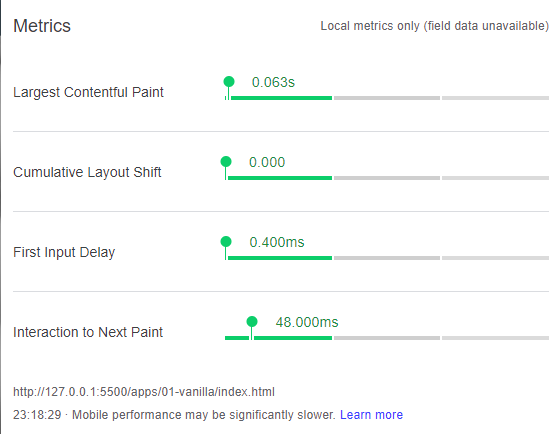
\includegraphics[width=0.45\textwidth]{01_desktop.png}
	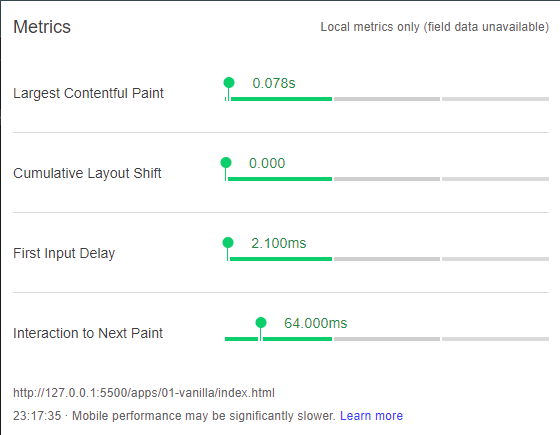
\includegraphics[width=0.45\textwidth]{01_mobile.png}
	\caption{Aplicația vanilla JavaScript, desktop și mobile}
	\label{fig:01-local}
\end{figure}

\begin{figure}[htbp]
	\centering
	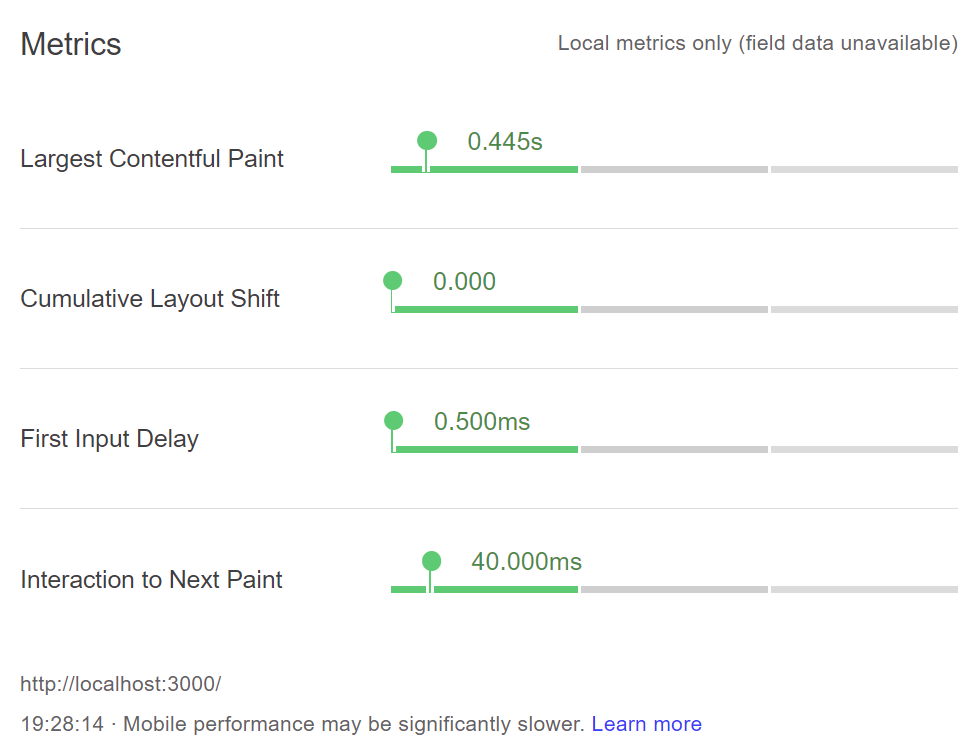
\includegraphics[width=0.45\textwidth]{02_desktop.png}
	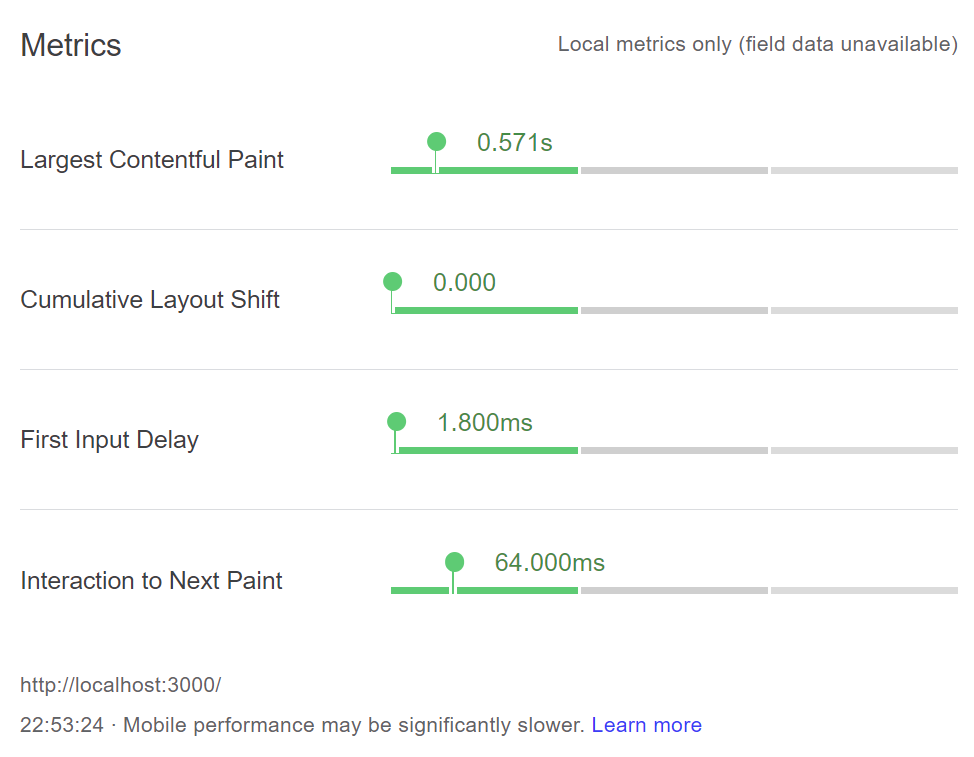
\includegraphics[width=0.45\textwidth]{02_mobile.png}
	\caption{Aplicația React, desktop și mobile}
	\label{fig:02-local}
\end{figure}

După deploy-ul aplicațiilor pe web hosting, am efectuat repetat procesul de evaluare a performanței cu ajutorul extensiei și am obținut următoarele rezultate:

\begin{figure}[htbp]
	\centering
	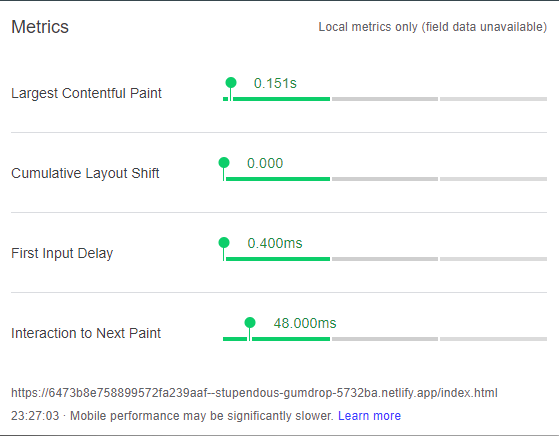
\includegraphics[width=0.45\textwidth]{01_desktop_deployed.png}
	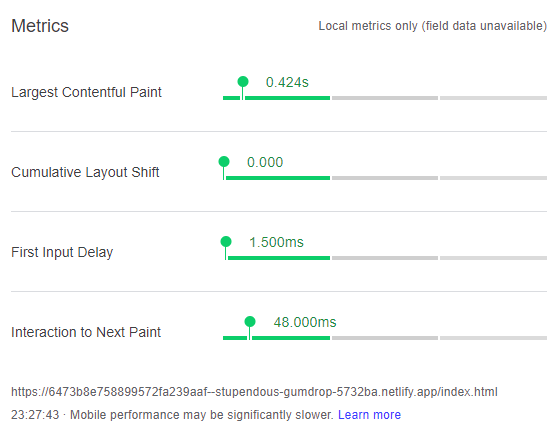
\includegraphics[width=0.45\textwidth]{01_mobile_deployed.png}
	\caption{Aplicația vanilla JavaScript, desktop și mobile}
	\label{fig:01-deployed}
\end{figure}

\begin{figure}[htbp]
	\centering
	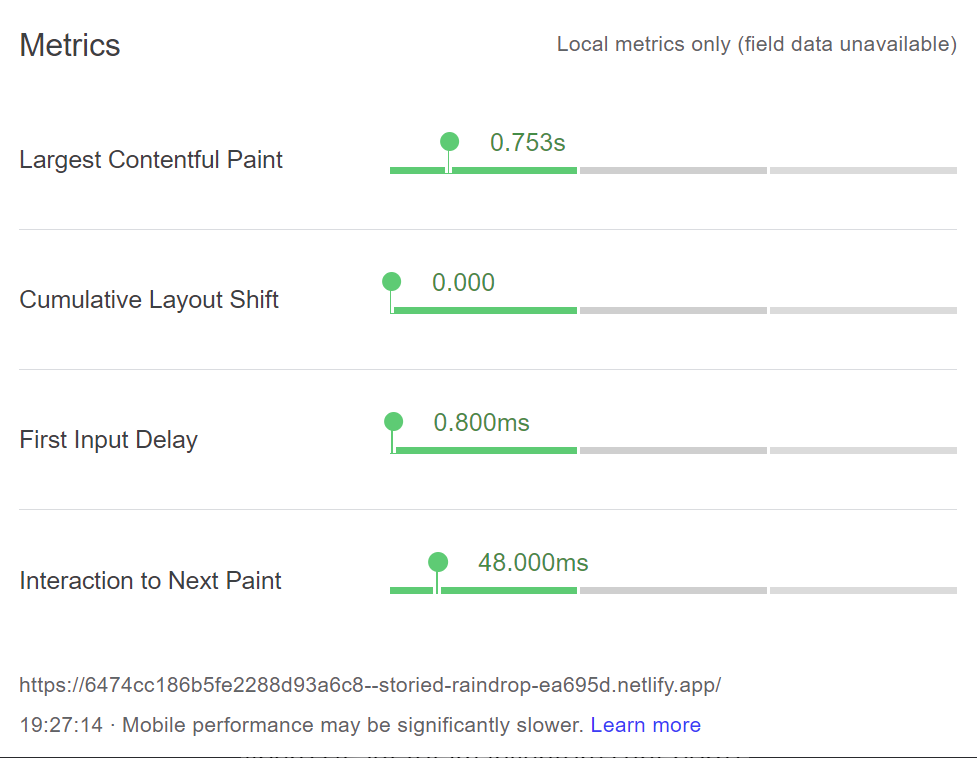
\includegraphics[width=0.45\textwidth]{02_desktop_deployed.png}
	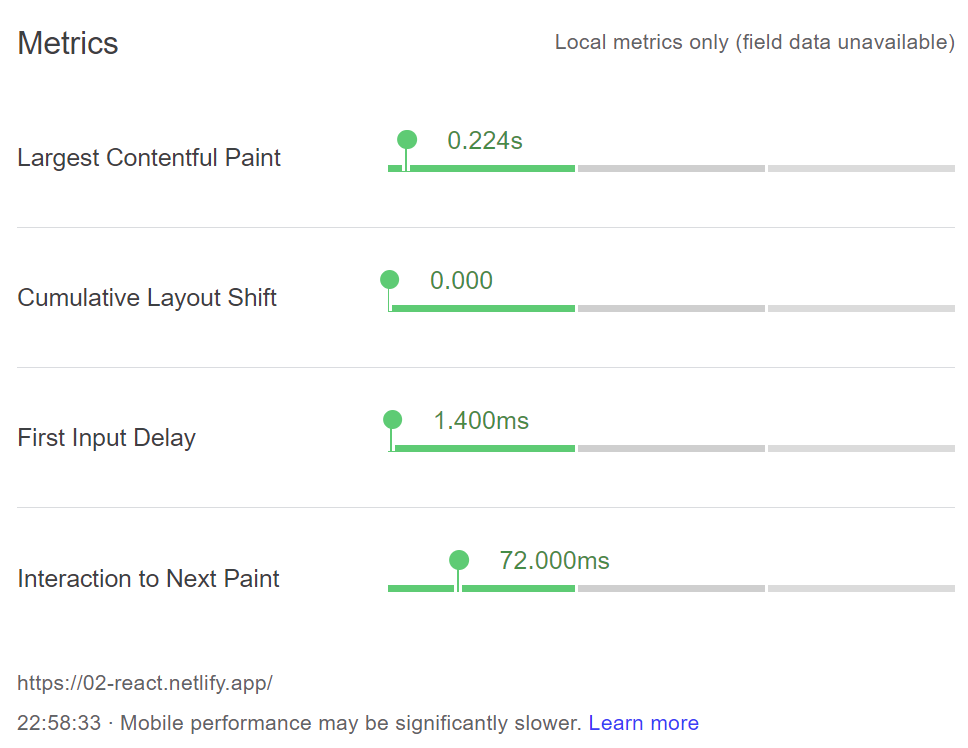
\includegraphics[width=0.45\textwidth]{02_mobile_deployed.png}
	\caption{Aplicația React, desktop și mobile}
	\label{fig:02-deployed}
\end{figure}

Procesul optimizat de randare al React-ului, arhitectura bazată pe componente și gestionarea eficientă a stărilor contribuie la îmbunătățirea metricilor de performanță. React utilizează un DOM virtual, care este o reprezentare în memorie a DOM-ului real. Acest lucru permite React-ului să actualizeze și să randeze eficient doar componentele necesare atunci când există modificări în starea aplicației.

Gestionarea eficientă a stărilor în React contribuie, de asemenea, la îmbunătățirea performanței. React folosește un flux unidirecțional al datelor și un concept numit "reconciliere" pentru a actualiza eficient interfața în funcție de modificările în starea aplicației.
\subsection{Lighthouse}

Cu ajutorul acestui tool, care este prezent în browserul Google Chrome, am generat rapoartele pentru ambele aplicații, atât în mediul local:

\begin{figure}[htbp]
	\centering
	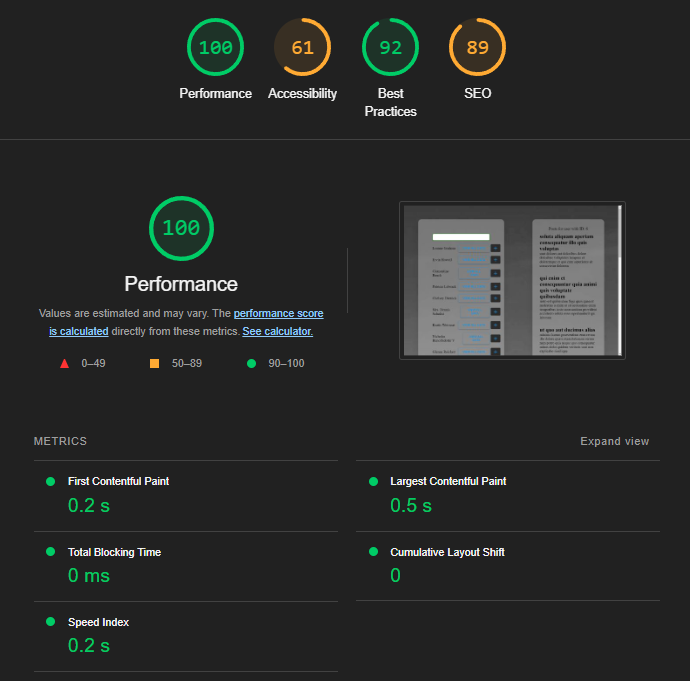
\includegraphics[width=0.45\textwidth]{01_desktop_lighthouse.png}
	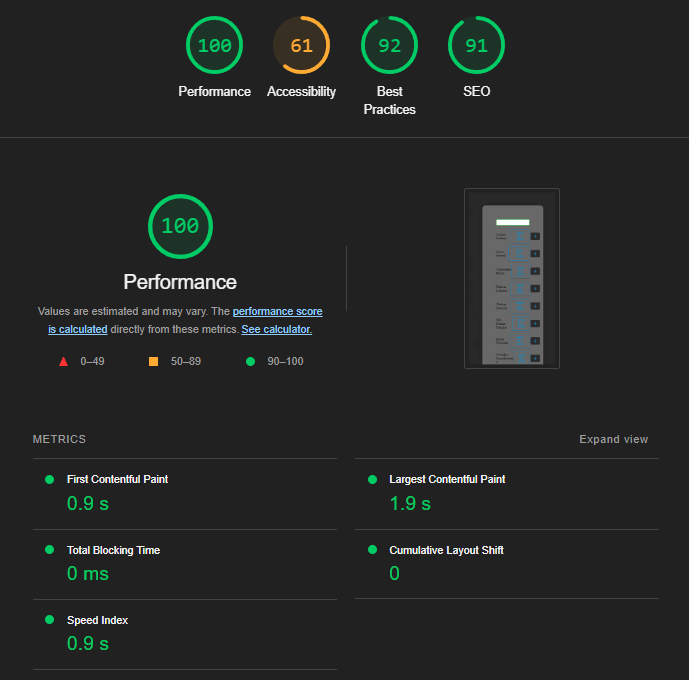
\includegraphics[width=0.45\textwidth]{01_mobile_lighthouse.png}
	\caption{Aplicația vanilla JavaScript, desktop și mobile}
	\label{fig:01-local-lighthouse}
\end{figure}

\begin{figure}[htbp]
	\centering
	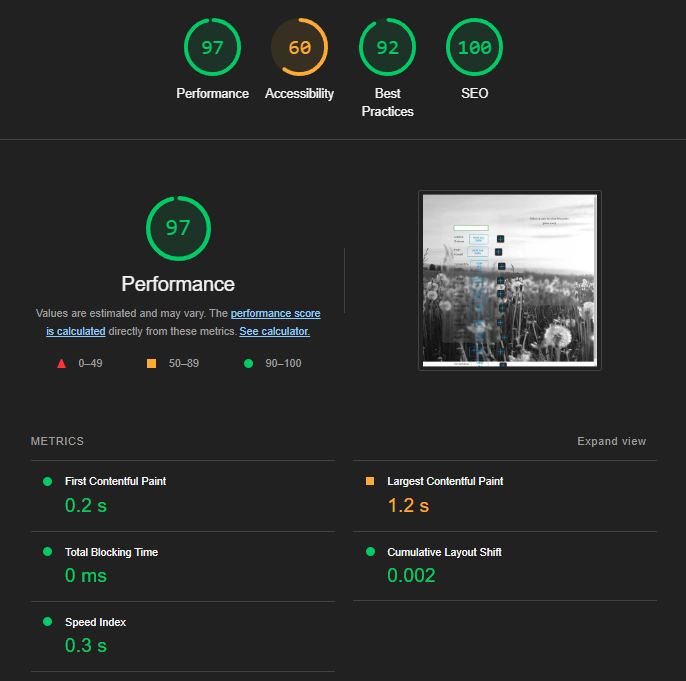
\includegraphics[width=0.45\textwidth]{02_desktop_lighthouse.png}
	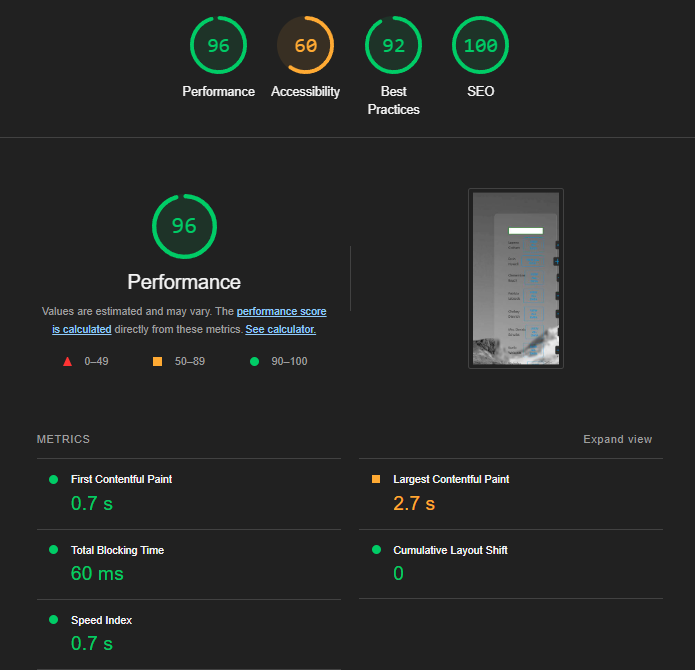
\includegraphics[width=0.45\textwidth]{02_mobile_lighthouse.png}
	\caption{Aplicația React, desktop și mobile}
	\label{fig:02-local-lighthouse}
\end{figure}

\newpage
cât și după deploy-ul pe hosting:

\begin{figure}[htbp]
	\centering
	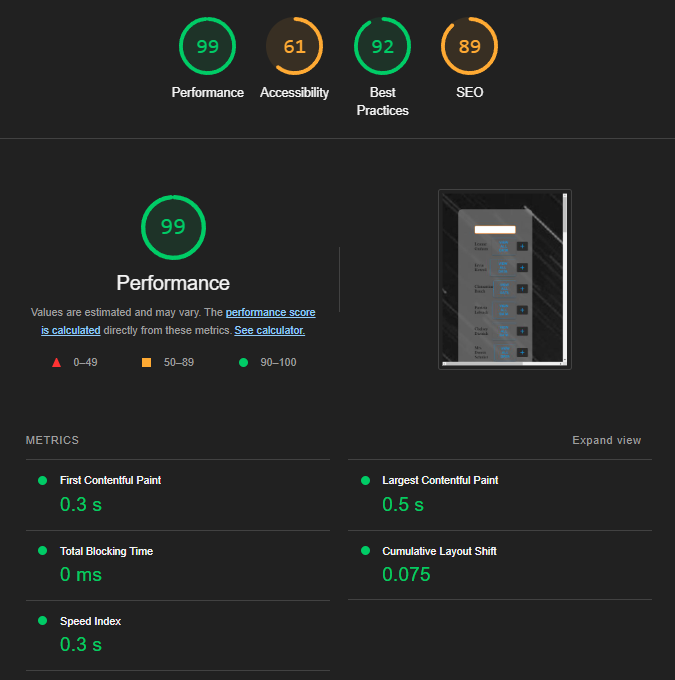
\includegraphics[width=0.45\textwidth]{01_desktop_deployed_lighthouse.png}
	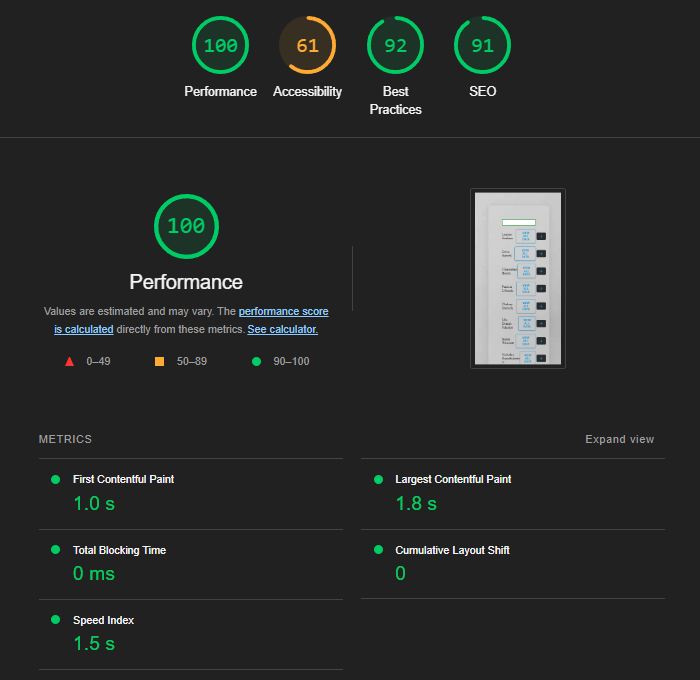
\includegraphics[width=0.45\textwidth]{01_mobile_deployed_lighthouse.png}
	\caption{Aplicația vanilla JavaScript, desktop și mobile}
	\label{fig:01-deployed-lighthouse}
\end{figure}

\begin{figure}[htbp]
	\centering
	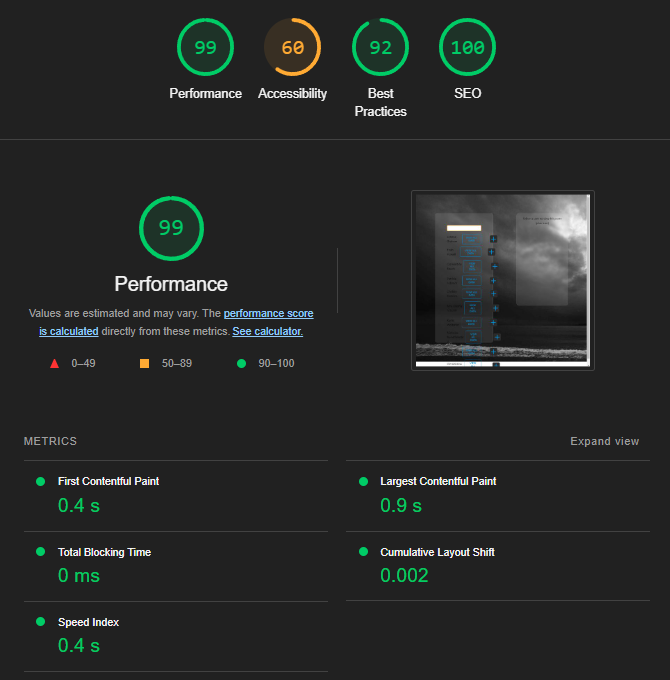
\includegraphics[width=0.45\textwidth]{02_desktop_deployed_lighthouse.png}
	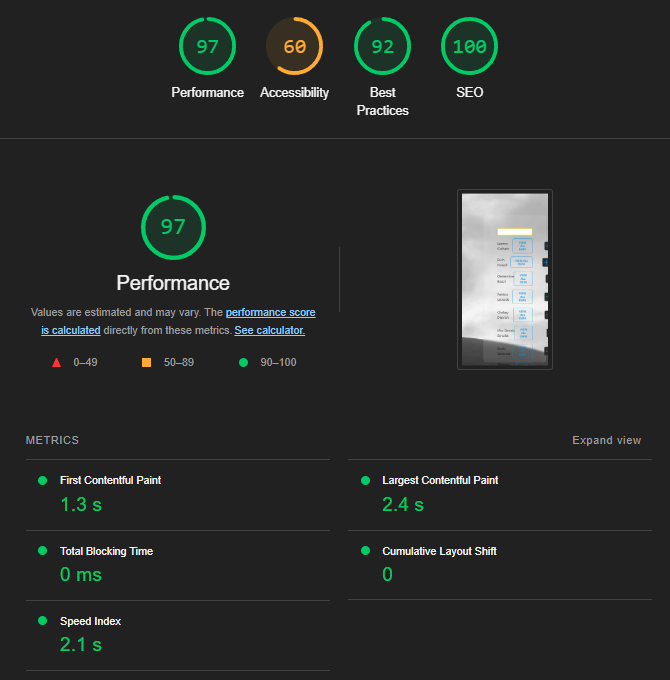
\includegraphics[width=0.45\textwidth]{02_mobile_deployed_lighthouse.png}
	\caption{Aplicația React, desktop și mobile}
	\label{fig:02-deployed-lighthouse}
\end{figure}

\subsection{PageSpeed Insights}

PageSpeed evaluează pagina atât pe dispozitive mobile, cât și pe desktop, atribuie un scor în funcție de performanța paginii și se oferă recomandări pentru îmbunătățire. Acest tool ia în considerare mai mulți factori care pot afecta performanța unei pagini, cum ar fi timpul de răspuns al serverului, cache-ul resurselor, optimizarea imaginilor, minificarea JavaScript și CSS și altele. De asemenea, acesta ia în considerare utilizarea celor mai bune practici și a ghidurilor de performanță web, cum ar fi reducerea resurselor care blochează randarea, optimizarea căii critice de randare și folosirea cache-ului browserului.

Rezultatele obținute pentru ambele aplicații sunt:

\begin{figure}[htbp]
	\centering
	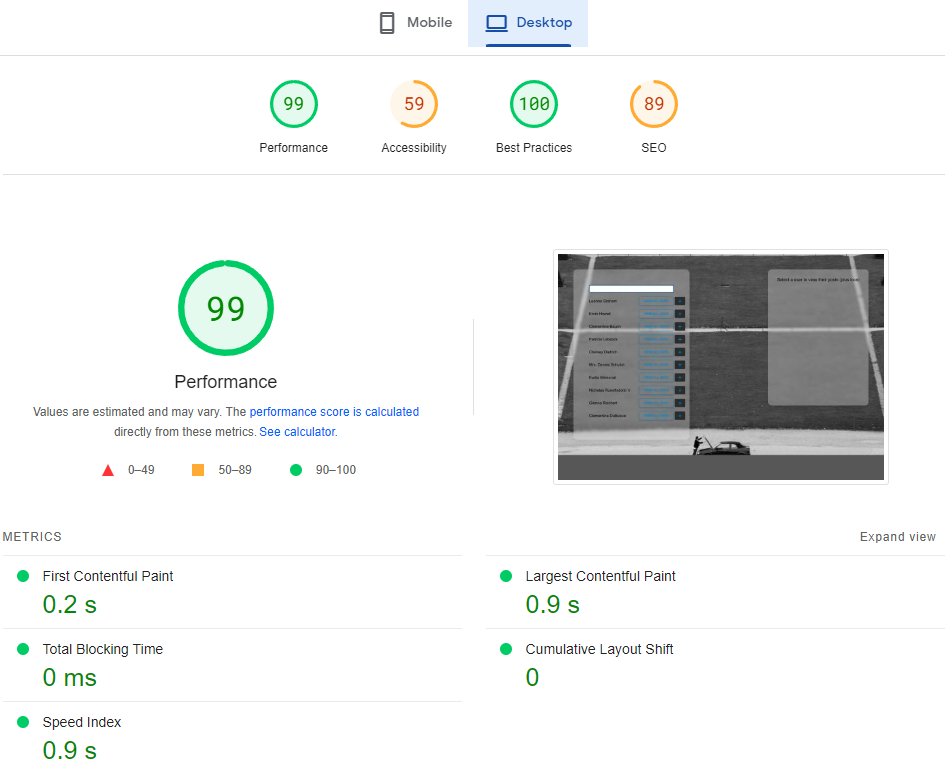
\includegraphics[width=0.45\textwidth]{01_desktop_pagespeed.png}
	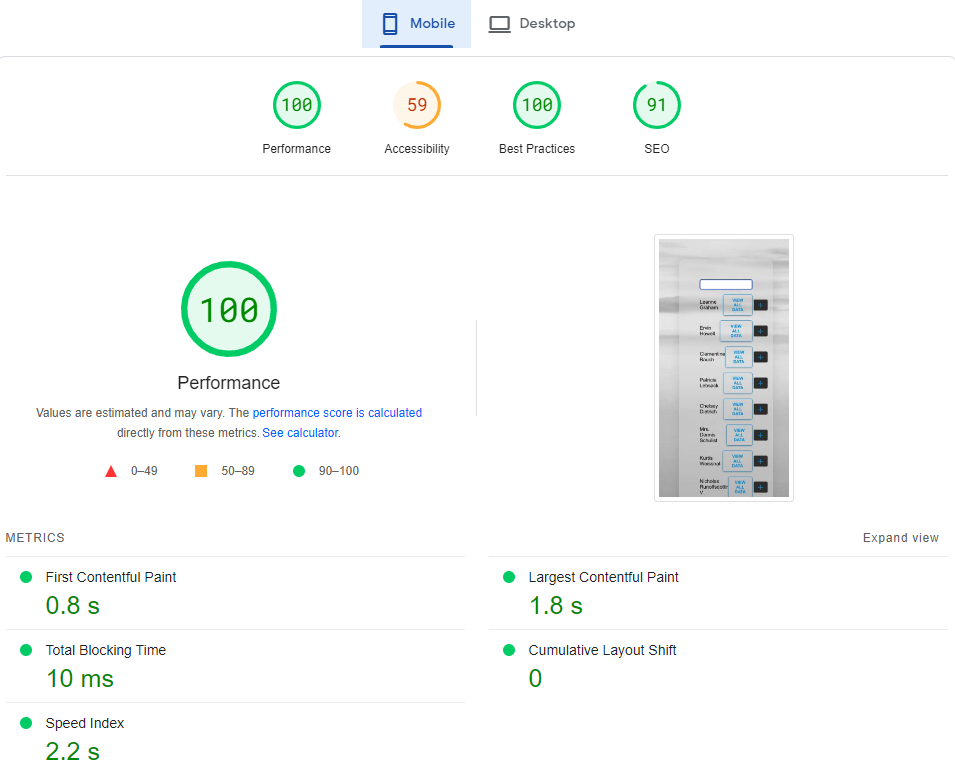
\includegraphics[width=0.45\textwidth]{01_mobile_pagespeed.png}
	\caption{Aplicația vanilla JavaScript, desktop și mobile}
	\label{fig:01-deployed-pagespeed}
\end{figure}

\begin{figure}[htbp]
	\centering
	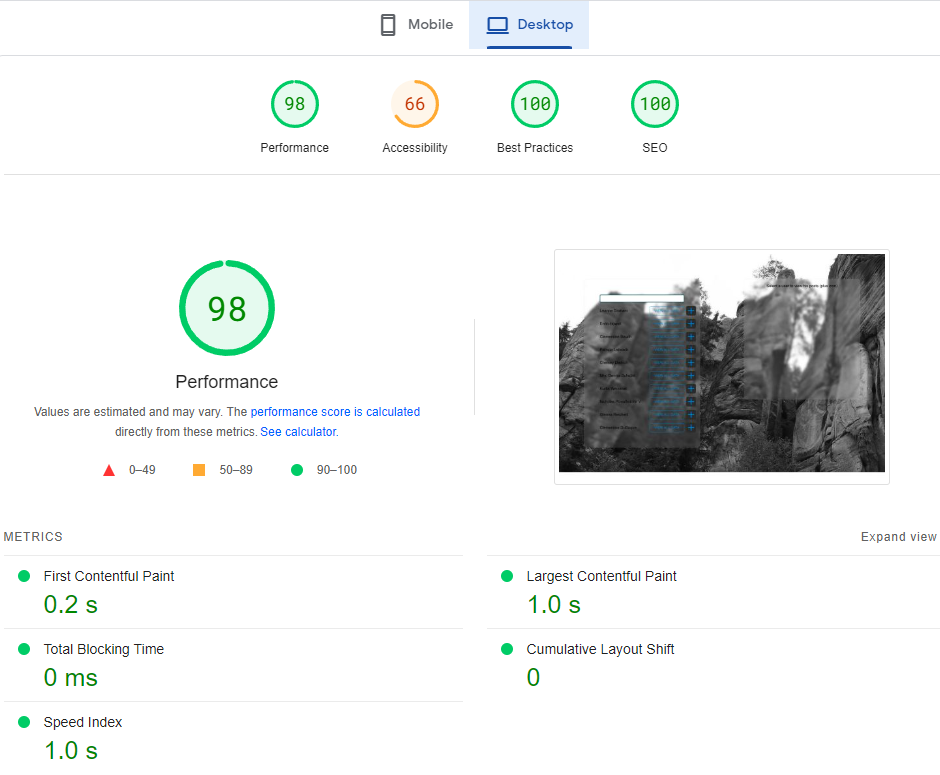
\includegraphics[width=0.45\textwidth]{02_desktop_pagespeed.png}
	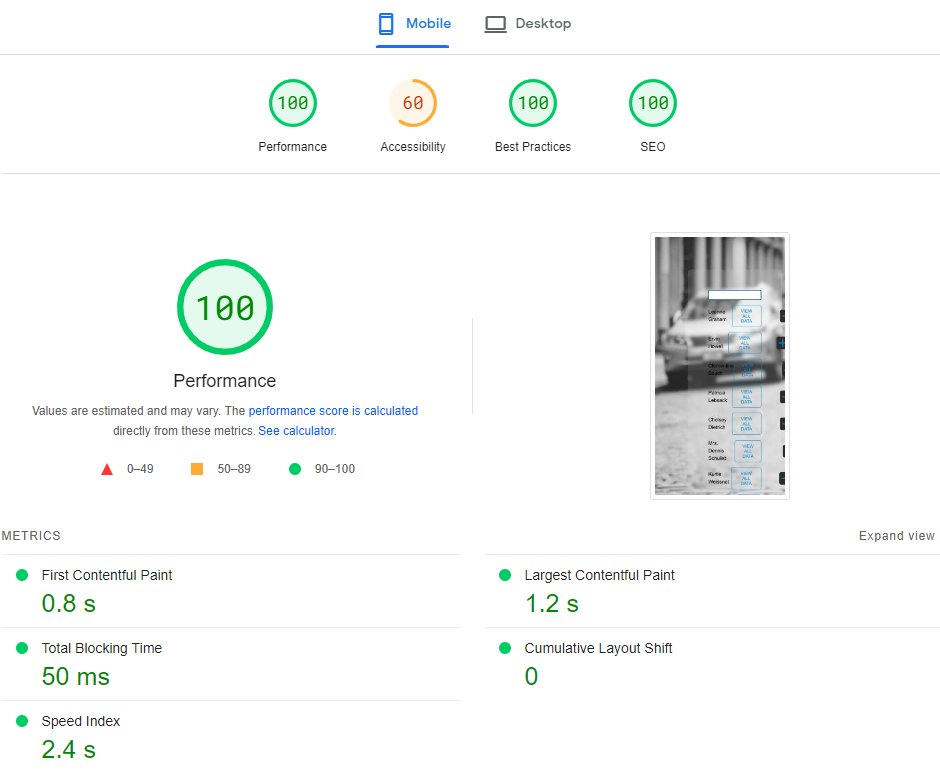
\includegraphics[width=0.45\textwidth]{02_mobile_pagespeed.png}
	\caption{Aplicația React, desktop și mobile}
	\label{fig:02-deployed-pagespeed}
\end{figure}

\section {Analiza rezultatelor}

Fiecare dintre metodele abordate are avantajele \c si dezavantajele sale. Vanilla JS este cel mai simplu de implementat, deoarece nu necesit\u a dependen\c te sau biblioteci suplimentare. React este un framework popular, care ofer\u a o abordare mai structurat\u a a dezvolt\u arii aplica\c tiilor web, dar necesit\u a un timp mai mare de implementare \c si configurare. Next.js \c si Gatsby sunt framework-uri construit pe React, care ofer\u a un set de func\c tionalit\u a\c ti suplimentare, care pot fi utile \^ in dezvoltarea unei aplica\c tii web, dar necesit\u a cuno\c stin\c te mai avansate de React \c si a specifica\c tiilor interne ale acestor framework-uri.


\subsection{U\c surin\c ta implement\u arii}
Din punct de vedere al utiliz\u arii, vanilla JS este cel mai proeminent, deoarece nu necesit\u a dependențe sau framework-uri suplimentare. Pentru a executa un cod JavaScript este destul\u a ad\u augarea unui tag \textit{\textless script\textgreater }   \^ in pagina HTML:
\begin{lstlisting}[caption={Exemplu de ad\u augare a unui script \^ in pagina HTML},captionpos=b]
	<script>
		const exemplu = "Hello World!";
	</script>
	\end{lstlisting}

sau adaugarea unui fi\c sier JavaScript separat, care poate fi inclus \^ in pagina HTML cu ajutorul aceluia\c si tag, dar cu specificarea loca\c tiei fi\c sierului:

\begin{lstlisting}[caption={Exemplu de ad\u augare a unui script dintr-un fi\c sier extern},captionpos=b]
	<script src="path/to/file.js"></script>
\end{lstlisting}

Aplica\c tiile create cu ajutorul framework-urilor React, necesit\u a pa\c si suplimentari pentru configurarea inițială a proiectului folosind \textit{create-react-app} sau configurarea manuală a unui mediu de dezvoltare. De asemenea, este necesar\u a instalarea dependențelor proiectului, care pot fi gestionate cu ajutorul unui package manager, cum ar fi \textit{npm} sau \textit{yarn}. React utilizează JSX - o sintaxă care combină JavaScript cu HTML, care necesită un preprocesor pentru a fi transformat în JavaScript valid.

\begin{lstlisting} [caption={Comparare sintax\u a JSX \c si JavaScript},captionpos=b]
	--- cod JSX
	const numbers = [1, 2, 3, 4, 5];
	const list = (
		<ul>
			{numbers.map((number) => (
			<li key={number}>{number}</li>
			))}
		</ul>
	);
	--- cod JavaScript
	const numbers = [1, 2, 3, 4, 5];
	const list = React.createElement("ul",null,
		numbers.map((number) =>
			React.createElement("li", { key: number }, number)
		)
	);

\end{lstlisting}

JSX îmbunătățește lizibilitatea codului prin utilizarea de cod similar HTML în cadrul JavaScript. Reprezentarea vizuală a structurii codului sporește ușurința de întreținere și debugging-ul.

Promovează o abordare modulară și bazată pe componente, care poate fi reutilizate, facilit\^and crearea și gestionarea elementelor de interfață. Componentele pot fi scrise direct în cadrul codului JavaScript, permițând o organizare eficientă a codului și reutilizabilitate.

\begin{lstlisting}[caption={Exemplu de component\u a React},captionpos=b]
	function Welcome(props) {
		return <h1>Hello, {props.name}</h1>;
	}
\end{lstlisting}

Next.js \c si Gatsby sunt framework-uri care se bazeaz\u a pe React, oferind un mediu de dezvoltare mai u\c sor, cu un set de funcționalități predefinite, cum ar fi server-side rendering, generarea de pagini statice, optimizarea imaginilor \c si altele. Acestea sunt utile pentru crearea de aplicații web complexe, care necesită o structură bine definită și o arhitectură scalabilă, \^ins\u a necesit\u a o perioad\u a de timp mai mare pentru a fi \^inv\u ațate \c si implementate.

\subsection{Performanța}

\^In urma analizei rezultatelor ob\c tinute cu ajutorul Web Vitals, rapoartelor generate de Lighthouse \c si PageSpeed Insights se poate obesrva faptul c\u a aplica\c tia construit\u a vanilla JavaScript este mai performant\u a, deoarece \^in intermediul unei aplica\c tii simple, modific\u arile directe asupra DOM sunt mai eficiente dec\^at utilizarea Virtual DOM-ului. De asemenea, aplica\c tiile ce pe baz\u a de React necesit\u a mai multe resurse pentru a rula, deoarece este nevoie de biblioteci suplimentare pentru a utiliza func\c tionalit\u a\c ti suplimentare precum server-side rendering, dynamic routing, optimizarea imaginilor, etc.

\subsection{SEO}

Vanilla JS nu oferă suport direct pentru optimizarea pentru motoarele de căutare. Implementarea SEO trebuie făcută manual, inclusiv gestionarea meta tag-urilor, structurarea conținutului și gestionarea URL-urilor.

React oferă suport pentru optimizarea pentru motoarele de căutare, prin intermediul unor biblioteci dedicate \c si necesită atenție suplimentară și cunoștințe SEO pentru a implementa aceste optimizări. Prin utilizarea React Helmet sau a altor biblioteci similare, este posibi\u a adăugarea meta tag-urilor relevante.

Next.js are abilități de optimizare pentru SEO încorporate. Oferă suport nativ pentru server-side rendering (SSR) - paginile vor fi pregătite și livrate către motoarele de căutare cu conținutul complet generat, facilitând astfel indexarea și clasificarea mai bună în rezultatele căutării. Next.js gestionează automat meta tag-urile dinamice pentru fiecare pagină și, de asemenea, facilitează generarea paginilor statice, care pot fi extrem de benefice pentru SEO.

Gatsby este un framework care pune accent pe performanță și optimizare pentru SEO. Prin generarea paginilor statice în avans, Gatsby oferă un avantaj semnificativ în ceea ce privește viteza de încărcare a paginilor și indexarea lor de către motoarele de căutare. Gatsby are, de asemenea, suport nativ pentru gestionarea meta tag-urilor și structurarea conținutului pentru a obține rezultate optime în SEO. De asemenea, Gatsby beneficiază de integrarea cu GraphQL, permițând încărcarea eficientă a datelor și gestionarea optimă a conținutului pentru SEO.

\chapter{Concluzii}

Această lucrare ofer\u a o perspectivă asupra tehnologiilor de randare și a impactului lor asupra aplicațiilor web din punct de vedere al performanței, optimizării \c si experienței utilizatorilor.
Este important de menționat faptul că performanța unei aplicații web nu se rezumă doar la tehnologia de randare utilizată, ci și la practicile de optimizare și îmbunătățire continuă. Utilizarea instrumentelor precum Lighthouse și PageSpeed Insights poate oferi informa\c tii valoroase pentru identificarea punctelor slabe și îmbunătățirea performanței unei aplicații web.

Alegerea tehnologiei de randare depinde de cerințele specifice ale aplicației proiectate. SSR oferă avantaje din punct de vedere al SEO, datorită faptului c\u a con\c tinutul HTML este generat direct pe server \c si este furnizat c\u atre motoarele de c\u autare, îmbunătățirea performanței încărcării inițiale a paginii, dar are dezavantaje în ceea ce privește interactivitatea, deoarece întreaga pagină trebuie reîncărcată pentru a actualiza conținutul. 

CSR, pe de altă parte, oferă o experiență mai interactivă, deoarece conținutul este generat în browser, dar are dezavantaje în ceea ce privește performanța încărcării inițiale a paginii, deoarece întregul JavaScript trebuie descărcat și executat înainte ca pagina să poată fi afișată.

SSG este o alternativă la SSR, care oferă avantajele SEO și performanța încărcării inițiale a paginii, dar nu oferă interactivitatea oferită de CSR. 

În ceea ce privește tehnologiile de randare, React oferă o experiență de dezvoltare mai bună, datorită faptului că este mai ușor de învățat și de utilizat, oferind unelte \textit{precum create-react-app}, care oferă un mediu de dezvoltare preconfigurat \c si sintax\u a cunoscut\u a, deoarece este bazat pe JavaScript. Beneficiile care le ofer\u a React sunt cel mai eviden\c tiate în aplicațiile complexe cu interfețe de utilizator dinamice și actualizări frecvente, unde virtual DOM și mecanismele eficiente de randare oferă un UX mai bun.

Vanilla JS, pe de altă parte, oferă o performanță mai bună, deoarece nu necesită biblioteci suplimentare, dar are o curba de învățare mai mare și necesită mai mult cod pentru a realiza aceleași funcționalități.

Cu toate acestea, este important de menționat că în aplicațiile mai simple sau în cazurile în care interactivitatea nu este un aspect major, JavaScript simplu poate fi mai performant datorită naturii sale. Vanilla JavaScript evită costurile suplimentare ale unui framework precum React și poate fi optimizat pentru cazuri de utilizare specifice, rezultând \^intr-o  execuție mai rapidă.

\section{Rezultatele obținute}

\^In urma analizei perfoman\c tei aplica\c tiilor construite, s-a constatat c\u a aplica\c tia ce utilizează vanilla JavaScript este mai performant\u a, deoarece nu necesit\u a rerand\u ari frecvente, iar aspectele dinamice ale aplica\c tiei sunt u\c sor de calculat \c si de actualizat. Aplica\c tiile ce au fost construite cu ajutorul React au o dimensiune mai mare, deoarece necesit\u a biblioteci suplimentare pentru a func\c tiona \c si trebuie configurate pentru a putea fi hostate pe web.

\^In aplicația ce utilizeaza vanilla JS, manipul\u arile DOM sunt realizate direct, iar \^in cazul unei aplica\c tii simple aceast\u a abordare direct\u a este mai eficient\u a dec\^at utilizarea React \c si virtual DOM, ce necesit\u a pa\c si suplimentari pentru actualizarea con\c tinutului.

Odată cu scalarea aplica\c tiei, React devine mai performant, iar codul mai u\c sor de men\c tinut, datorit\u a arhitecturii sale bazate pe componente reutilizabile \c si alte unelte de dezvoltare predefinite precum hook-urile, ce simplifică implementarea, actualizarea \c si scalarea optim\u a a func\c tionalit\u a\c tilor necesare.

\section {Direcții viitoare de cercetare}

În timp ce studiul actual s-a concentrat pe compararea performanței JavaScript-ului simplu (Vanilla), React, Next.js și Gatsby într-o aplicație web relativ simplă, există mai multe direcții pentru cercet\u ari ulterioare, care pot extinde înțelegerea asupra acestor tehnologii de randare în scenarii mai complexe. Prin investigarea acestor direcții, putem obține o perspectivă mai profundă asupra punctelor forte și limitărilor fiecărei tehnologii și a performanței acestora în aplicații web complexe, cu conținut dinamic \c si actualiz\u ari frecvente ale componentelor.

Prin creșterea complexității și a dimensiunii aplicației, inclusiv ad\u augarea mai multor pagini, va fi posibi\u a evaluarea modului în care fiecare tehnologie gestionează sarcina de lucru suplimentară. Această analiză ar ajuta la determinarea dacă anumite tehnologii sunt mai potrivite pentru aplicații de mari dimensiuni și ar dezvălui eventuale restricții de performanță care pot apărea.

Acest studiu sa axat pe utilizarea vanilla JS, React, Next.js și Gatsby, \^ins\u a există numeroase framework-uri \c si tehnologii de randare. Cercet\u arile ulterioare ar putea extinde comparația pentru a include alte framework-uri sau biblioteci, cum ar fi Angular, Vue.js sau Svelte \c si tehnologii de randare precum ISR (\textit{Incremental Static Regeneration}), care este o variant\u a \^imbun\u at\u a\c tit\u a a SSG, \^in care paginile statice se pot regenera pe server la cerere, f\u ar\u a necesitatea de rebuild a \^intregii aplica\c tii. 

Prin includerea unui spectru mai larg de tehnologii de randare, putem obține o perspectivă mai largă asupra performanței acestora și a modului în care se compară cu cele evaluate în acest studiu.



\renewcommand{\bibname}{Bibliografie}

\bibliographystyle{Plain} % Plain, Abbrv, Unsrt, Alpha
\addcontentsline{toc}{chapter}{Bibliography}

\begin{thebibliography} {12}
	\bibitem{serversiderendering} John H. Conway. Server-side rendering versus client-side rendering: A performance comparison. ACM, 2015

	\bibitem {pwa} Maximiliano Firtman. Progressive Web Apps: The Future of Web Development. O'Reilly Media, 2017

	\bibitem{serversiderenderingreactredux} Jason W. Bock. Server-Side Rendering with React and Redux. Packt Publishing, 2018

	\bibitem{bernslee90} Tim Berners-Lee. The WorldWideWeb browser. W3C, 1990

	\bibitem{html} Tim Berners-Lee, Daniel Connolly. Hypertext markup language (html). CERN, Geneva, Switzerland, 1993

	\bibitem{metrics} Serge Demeyer. Software Metrics - ansymore.uantwerpen.be, 2017

	\bibitem{benefitsserverrendering} Alex Grigoryan. The Benefits of Server Side Rendering Over Client Side Rendering - https://medium.com/walmartlabs/the-benefits-of-server-side-rendering-over-client-side-rendering-5d07ff2cefe8, 2017

	\bibitem{vuewangularreact} Benjamin Jakobus. VueJS vs Angular vs ReactJS with Demos - http://www.dotnetcurry.com/vuejs/1372/vuejs-vs-angular-reactjs-compare, 2017

	\bibitem{fireship} Jeff Delaney. 10 Rendering Patterns for Web Apps, 2023

	\bibitem{clientsidevssercerside} Sergey Laptick. Client Side vs Server Side UI Rendering. Advantages and Disadvantages - https://blog.webix.com/client-side-vs-server-side-ui-rendering/, 2017

	\bibitem{webdev} Jason Miller, Addy Osmani. Rendering on the Web - https://web.dev/rendering-on-the-web/, 2019

	\bibitem{improve-ssr-speed} Anna Monus. What Is Server-side Rendering And How Does It Improve Site Speed?
	- https://www.debugbear.com/blog/server-side-rendering, 2019

	\bibitem{google-bouncing-rate} Google/SOASTA Research - https://www.thinkwithgoogle.com/marketing-strategies/app-and-mobile/mobile-page-speed-new-industry-benchmarks-load-time-vs-bounce/, 2017

\end{thebibliography}


\appendix % begin appendix part

\chapter{Glosar}


\section{Acronime}

\begin{table} [H]
	\begin{tabular} {|  l | L{10cm} |}
		\hline
		SSR & Server side rendering      \\ [0.2ex]
		\hline
		CSR & Client side rendering      \\ [0.2ex]
		\hline
		SSG & Static server generation   \\ [0.2ex]
		\hline
		UX  & User experience            \\ [0.2ex]
		\hline
		UI  & User interface             \\ [0.2ex]
		\hline
		LCP & Largest contentful paint   \\ [0.2ex]
		\hline
		FID & First input delay          \\ [0.2ex]
		\hline
		CLS & Comulative layout shift    \\ [0.2ex]
		\hline
		SEO & Search engine optimization \\ [0.2ex]
		\hline
		JS  & JavaScript                 \\ [0.2ex]
		\hline
	\end{tabular}
	\caption{Tabelă de acronime}
	\label{table:acron}
\end{table}

% end appendix part

\end{document}
